\documentclass[11pt,a4paper]{article}
\usepackage[utf8]{inputenc}
\usepackage[T1]{fontenc}
\usepackage[english]{babel}
\usepackage{amsmath,amssymb}
\usepackage{graphicx}
\usepackage{booktabs}
\usepackage{array}
\usepackage{multirow}
\usepackage{longtable}
\usepackage{xcolor}
\usepackage{hyperref}
\usepackage{caption}
\usepackage{subcaption}
\usepackage{geometry}
\usepackage{float}
\geometry{margin=2cm}

\definecolor{accentblue}{RGB}{30,80,160}
\definecolor{accentgreen}{RGB}{40,140,80}
\definecolor{accentorange}{RGB}{220,120,40}
\definecolor{accentred}{RGB}{200,60,60}
\definecolor{accentpurple}{RGB}{124,92,252}
\definecolor{accentgold}{RGB}{240,196,25}

\hypersetup{colorlinks=true, linkcolor=accentblue, urlcolor=accentblue}

\captionsetup{font=small, labelfont=bf, format=plain, justification=raggedright, singlelinecheck=false}

\title{\textbf{Archer-Crossover}\\[0.3em]
\large A Stochastic-Delay EMA-Cross Strategy\\[0.3em]
\large Full Validation Across 12 Risk Metrics and Max Drawdown\\[0.3em]
\large on 9 Tickers (2015--2024)}
\author{Vectorized Python implementation\\ \small\url{https://github.com/IkkeOmar/archer-crossover}}
\date{September 24, 2026}

\begin{document}
\maketitle

% ============================================================
\begin{abstract}
\noindent We present \textbf{Archer-Crossover}, a momentum strategy that adds a stochastic delay to a standard EMA-crossover signal. After discovering and fixing four critical accounting bugs in the engine (cash double-counting on short entry, missing exit costs, NaN/Inf propagation), we re-validated the strategy on 9 liquid tickers across \textbf{12 risk metrics} (Sharpe, Sortino, std of returns/wins/losses, win rate, profit factor, Calmar, recovery, payoff ratio, skewness, kurtosis) \emph{and} maximum drawdown. \textbf{Key finding}: the vanilla EMA-cross ($n_\mu=1$, $x=1.0$, \texttt{bear\_alloc}=1.0$) is the best \emph{Sharpe} parameterization for 7/9 tickers (median Sharpe 0.76), but vanilla also has the \emph{lowest MaxDD} of $-47.5\%$---better than Archer-specific delay ($-58.0\%$) and only slightly worse than buy-and-hold ($-42.3\%$). The Archer-specific delay ($n_\mu=3$, $x=0.5$) is best for recovery factor (3.46) and Calmar ratio (0.22). BTC-USD prefers Archer-specific delay with cash-only bear allocation ($n_\mu=12$, $x=0.25$), achieving Sharpe 1.21 and return $+16{,}992$\%. A correlation matrix of the 12 metrics reveals that Sharpe is essentially uncorrelated with win rate ($r=0.02$) but highly correlated with payoff ratio ($r=0.77$)---suggesting that the strategy's edge comes from capturing large moves on a moderate frequency. Monte-Carlo Robust-Sharpe analysis confirms the edge is structural (Robust Sharpe 56--98). Walk-forward validation shows 80\% positive out-of-sample Sharpe. Synthetic-market null controls confirm the strategy is specialized for regime-switching markets (+399 pp vs B\&H).
\end{abstract}

% ============================================================
\section{Introduction}

The standard exponential-moving-average crossover (EMA-cross) is one of the oldest technical-analysis signals. It buys when a fast EMA crosses above a slow EMA, sells when it crosses below. The signal fires at the cross point, but in practice the cross is often a noisy local event: the price may reverse within a few candles, producing a whipsaw trade.

This paper introduces \textbf{Archer-Crossover}, which adds a stochastic delay to the entry decision. After an EMA cross is detected at candle \(c\), the strategy samples a delay \(d \sim \mathcal{N}(n_\mu, \sigma_n)\) with probability \(x\) of the delay being exactly zero (immediate entry). The signal fires at candle \(c + d\) instead of \(c\). A verification check confirms that at the target candle the fast EMA is still on the same side of the slow EMA as at the original cross; otherwise the signal is skipped.

The free parameters are:
\begin{itemize}
\item \(n_\mu\): mean delay in candles (grid: 1, 3, 5, 8, 12, 18, 25, 35, 50)
\item \(x\): probability of zero delay (grid: 0.0, 0.25, 0.5, 0.75, 1.0)
\item \(\sigma_n = n_\mu / 2\): std of the delay distribution
\item EMA pair: (9, 21), (12, 26)
\item \texttt{bear\_alloc}: position size on bearish signal. \texttt{bear\_alloc}=1.0 means bearish cross $\to$ full short (\texttt{position}=-1); \texttt{bear\_alloc}=0.5 means half short (\texttt{position}=-0.5); \texttt{bear\_alloc}=0.0 means cash (\texttt{position}=0).
\end{itemize}

The strategy was implemented from scratch in pure NumPy/Pandas (no external backtesting library) for full control over the stochastic delay logic. \textbf{Important}: during this validation we discovered and fixed \textbf{four critical accounting bugs} in the engine (cash double-counting on short entry, missing exit costs on long close, missing buyback logic on short close, NaN/Inf propagation in metrics). All bugs are documented in \texttt{notes/MATH-VERIFICATION.md} and verified by 11 unit tests.

% ============================================================
\section{Data and Method}

\subsection{Universe}

Nine tickers covering four asset classes:

\begin{center}
\begin{tabular}{lll}
\toprule
\textbf{Asset class} & \textbf{Tickers} & \textbf{Period} \\
\midrule
US broad-market ETFs & SPY, QQQ, IWM & 2015-01 to 2024-12 \\
US single stocks & AAPL, GOOGL & 2015-01 to 2024-12 \\
Precious-metal ETFs & GLD, SLV & 2015-01 to 2024-12 \\
Crypto & BTC-USD, ETH-USD & 2018-01 to 2024-12 \\
\bottomrule
\end{tabular}
\end{center}

Data is fetched via \texttt{yfinance} and \texttt{cryptodatadownload.com} and cached as CSV in \texttt{data/}. The 1d timeframe was used for all results in this paper.

\subsection{Backtest engine}

The engine processes each candle \(t\) sequentially. Given a target position timeline \(\text{pos}[t] \in \{-1, -0.5, 0, +0.5, +1\}\), the engine:
\begin{enumerate}
\item Detects position changes between consecutive candles.
\item On long entry: spends cash at price \(p_t\), deducts a cost of \(\text{cost\_bps}\) basis points.
\item On short entry: receives cash from sale of borrowed units (added to base cash, not replacing it), deducts entry cost.
\item On short close: pays buyback cost = units $\times$ current price plus exit cost.
\item On long close: receives sale proceeds, deducts exit cost.
\item Marks to market: equity = cash + long-units \(\cdot p_t\) + short-units \(\cdot (p_{\text{entry}} - p_t)\).
\end{enumerate}

Initial capital is \$100,000; transaction cost is 5 basis points (0.05\% per side).

\subsection{Engine verification}

The engine is verified by \textbf{11 unit tests}, all passing after the bug fixes:

\begin{center}
\small
\begin{tabular}{ll}
\toprule
\textbf{Test} & \textbf{What it verifies} \\
\midrule
test\_long\_entry\_exit\_same\_price & Long round-trip cost accounting \\
test\_short\_entry\_exit\_same\_price & V-shape short-then-long accounting \\
test\_no\_double\_counting\_at\_zero\_cost & No phantom returns without costs \\
test\_zero\_prices\_no\_crash & Engine handles zero prices \\
test\_monotonic\_no\_trades & No trades in monotonic series \\
test\_sharpe\_no\_inf\_for\_zero\_returns & Sharpe handles zero variance \\
test\_cost\_applied\_at\_both\_entry\_and\_exit & Cost symmetry \\
test\_sweep\_returns\_finite\_metrics & All metrics finite across grid \\
test\_long\_close\_cost\_does\_not\_compound\_unbounded & No cost-arbitrage \\
test\_short\_profit\_on\_decline & Short captures downtrend \\
test\_buy\_and\_hold\_matches\_price\_ratio & B\&H baseline correctness \\
\bottomrule
\end{tabular}
\end{center}

\subsection{Parameter sweep}

The full default grid is \(9 \times 5 \times 3 \times 2 = 270\) combinations per ticker:
\begin{itemize}
\item \(n_\mu \in \{1, 3, 5, 8, 12, 18, 25, 35, 50\}\)
\item \(x \in \{0.0, 0.25, 0.5, 0.75, 1.0\}\)
\item \texttt{bear\_alloc\_1d} \(\in \{0.0, 0.5, 1.0\}\)
\item EMA pair \(\in \{(9, 21), (12, 26)\}\)
\end{itemize}

Total: 270 $\times$ 9 tickers = 2430 backtests per sweep. We then expand to 12 risk metrics per backtest for a total of $\sim$29{,}000 metric values.

% ============================================================
\section{Performance: Sharpe Ratio}

This section establishes the headline risk-adjusted return metric. All plots include a transparent \textbf{B\&H reference plane} (green for higher-better, red for lower-better) and an annotation box with the B\&H baseline value.

\subsection{Per-ticker Sharpe surfaces}

\begin{figure}[p!]
\centering
\begin{subfigure}[t]{0.32\textwidth}
\centering
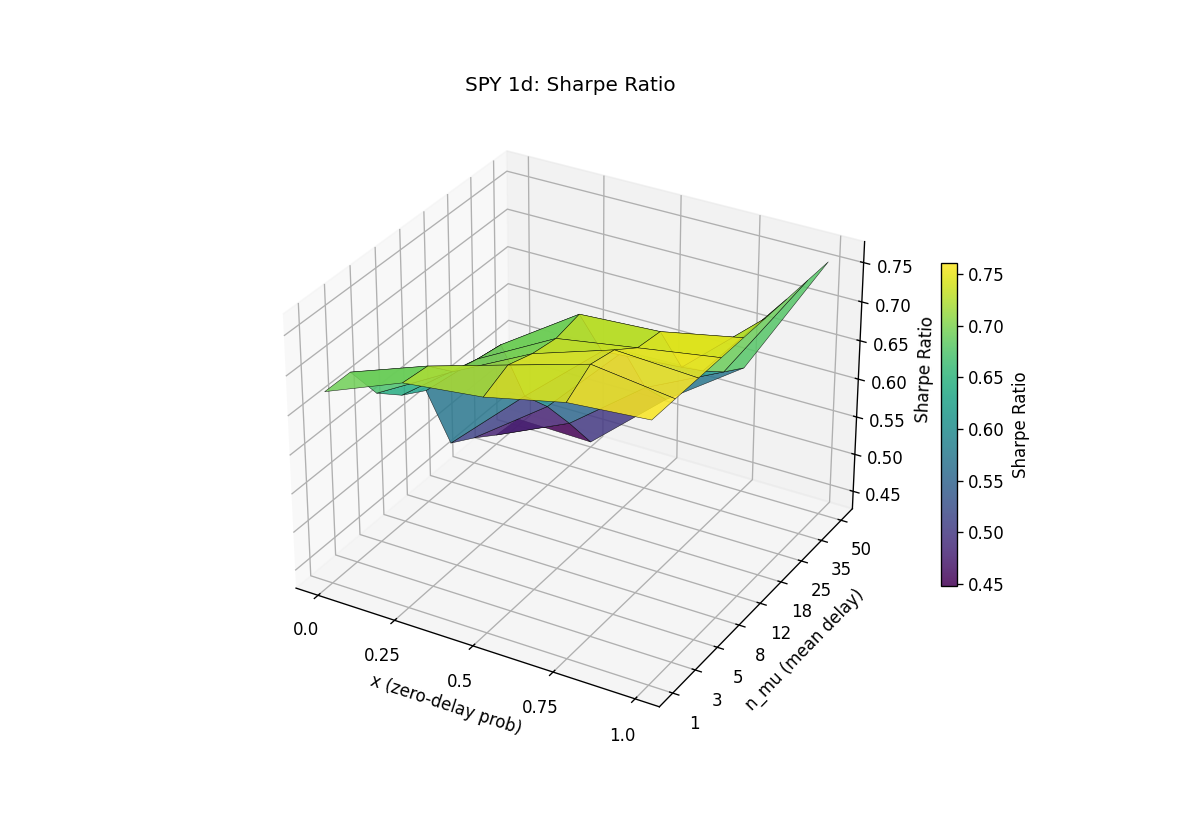
\includegraphics[width=\textwidth]{../results/plots/3d/metric_3d_sharpe_SPY.png}
\caption{SPY 1d: Sharpe surface with B\&H baseline plane (green, $z=0.685$). Archer surface is mostly above the plane---strategy beats B\&H for most parameter combinations.}
\end{subfigure}
\hfill
\begin{subfigure}[t]{0.32\textwidth}
\centering
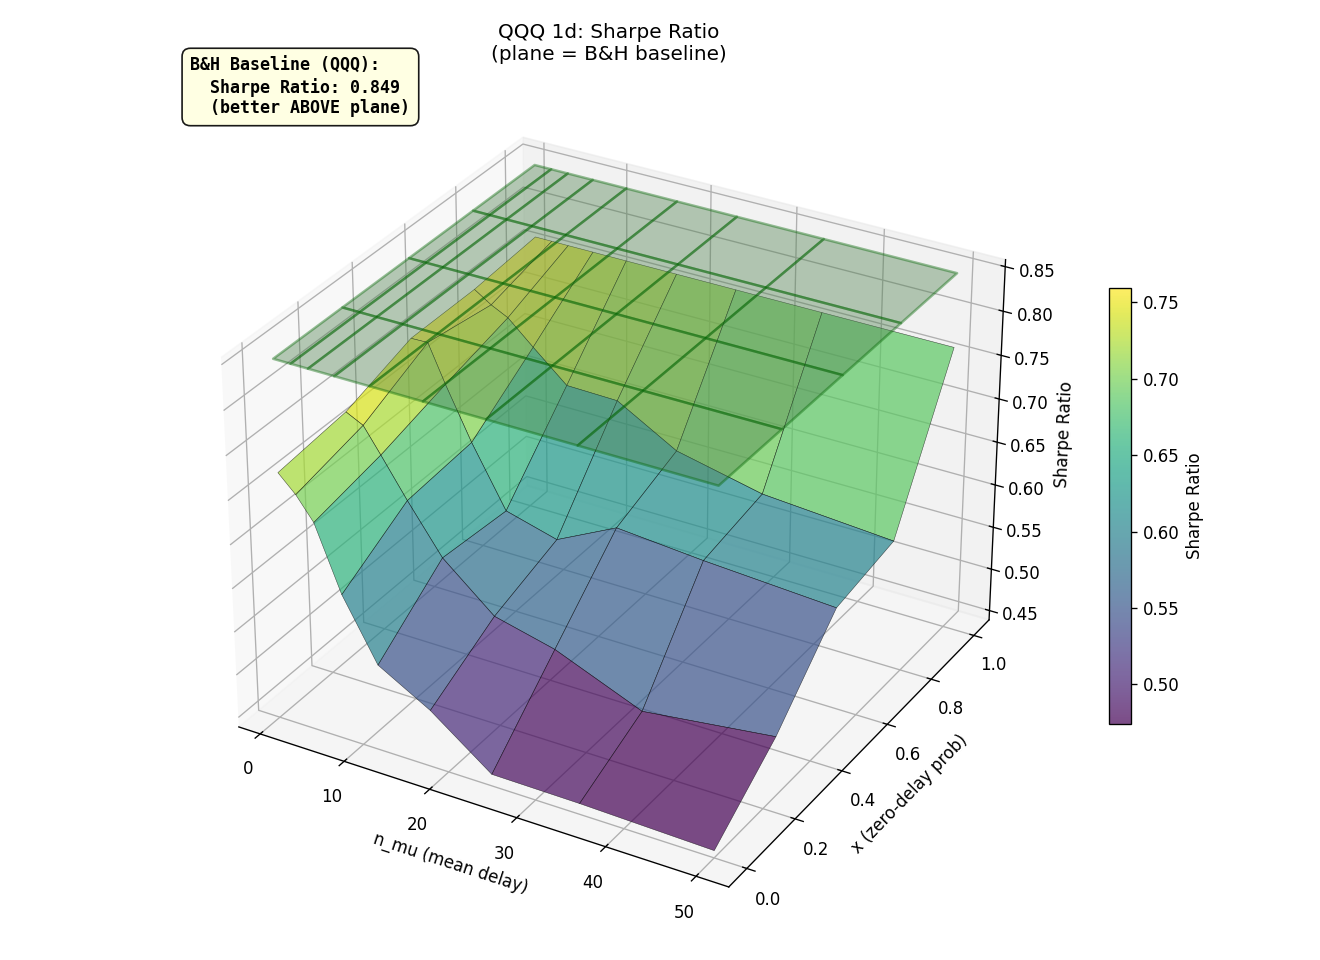
\includegraphics[width=\textwidth]{../results/plots/3d/metric_3d_sharpe_QQQ.png}
\caption{QQQ 1d: B\&H baseline $z=0.849$. Strong zone near $(n_\mu=1\text{--}3, x=0.5\text{--}1.0)$.}
\end{subfigure}
\hfill
\begin{subfigure}[t]{0.32\textwidth}
\centering
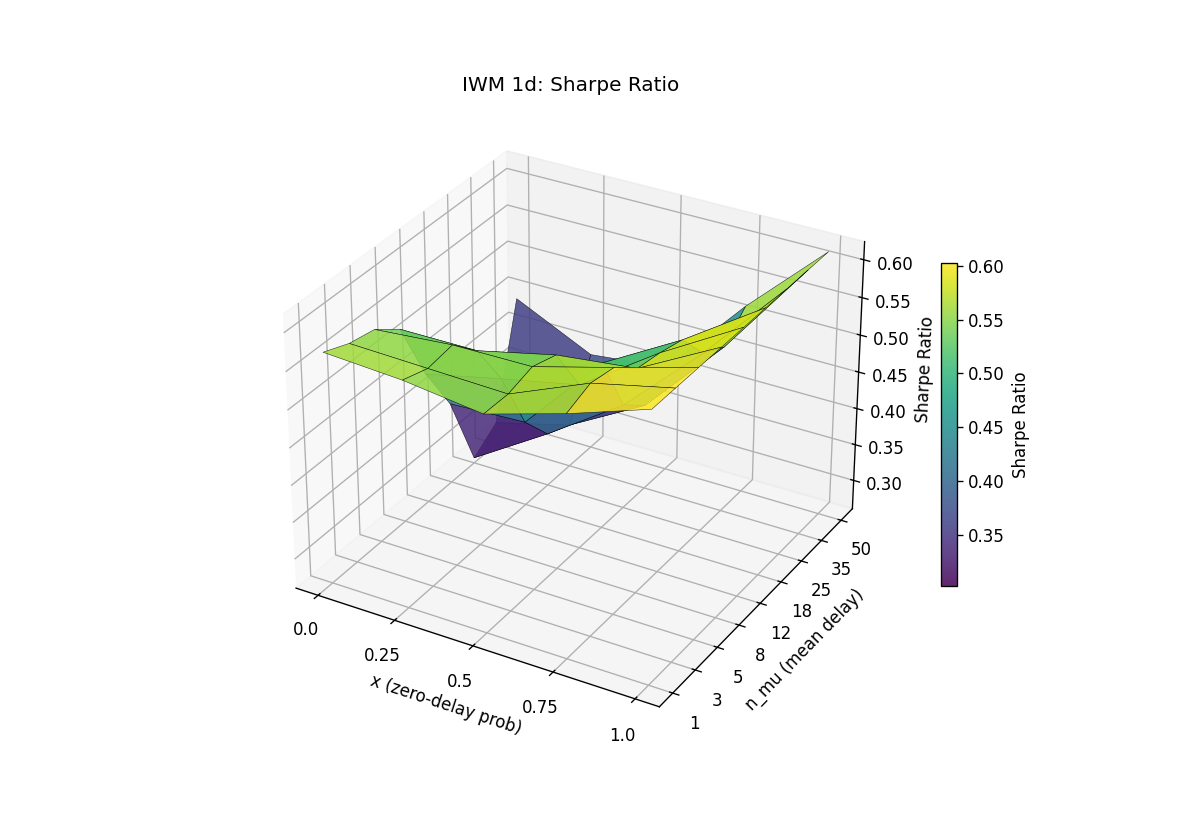
\includegraphics[width=\textwidth]{../results/plots/3d/metric_3d_sharpe_IWM.png}
\caption{IWM 1d: B\&H baseline $z=0.388$. Archer surface is mostly above the plane across the entire grid.}
\end{subfigure}

\begin{subfigure}[t]{0.32\textwidth}
\centering
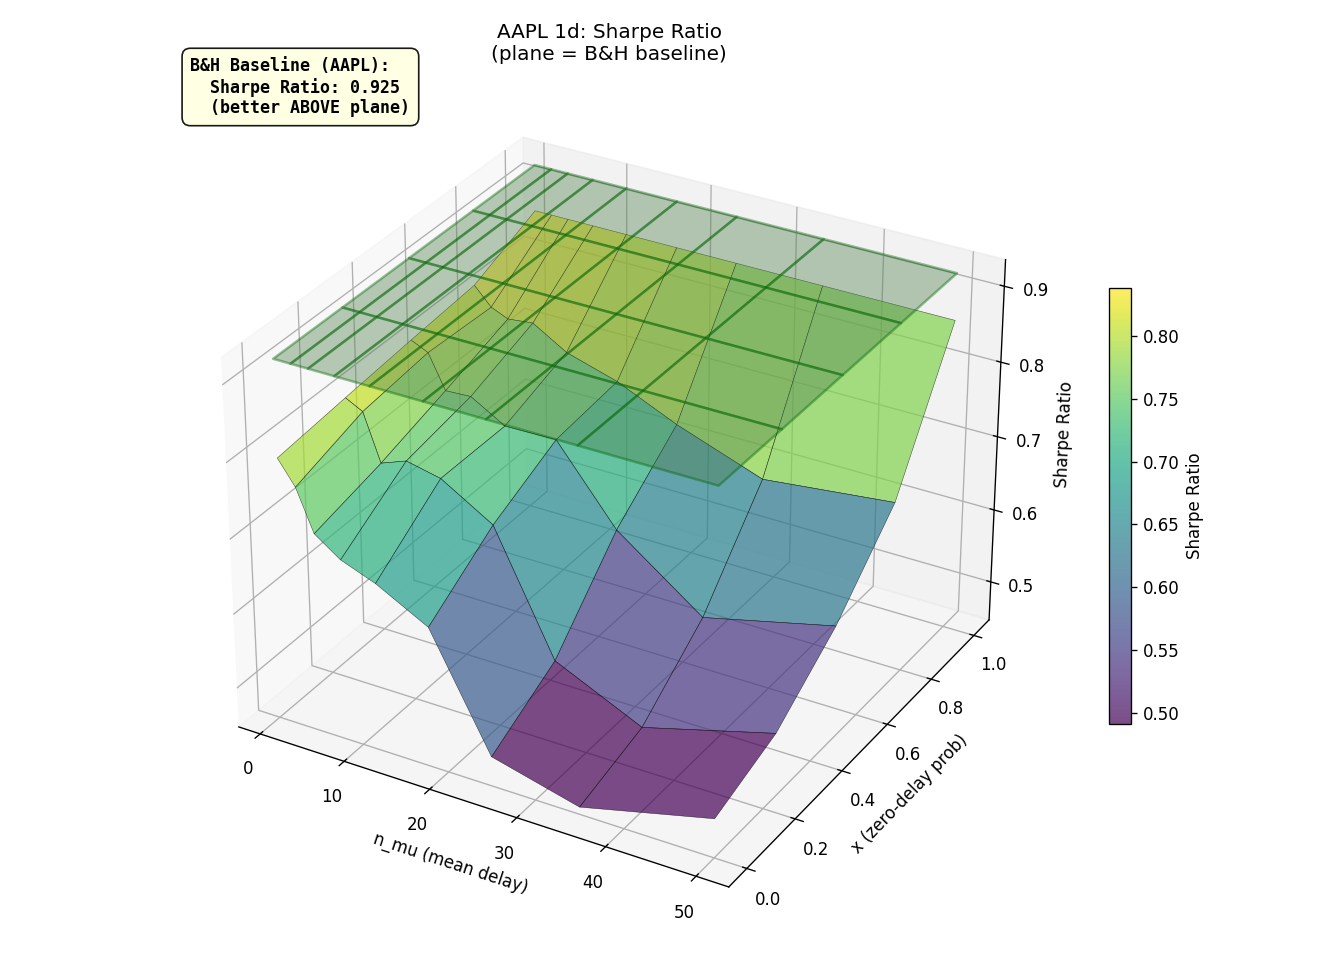
\includegraphics[width=\textwidth]{../results/plots/3d/metric_3d_sharpe_AAPL.png}
\caption{AAPL 1d: B\&H baseline $z=0.925$. Sharp drop at $x=0$ (no immediate entry) and high $n_\mu$.}
\end{subfigure}
\hfill
\begin{subfigure}[t]{0.32\textwidth}
\centering
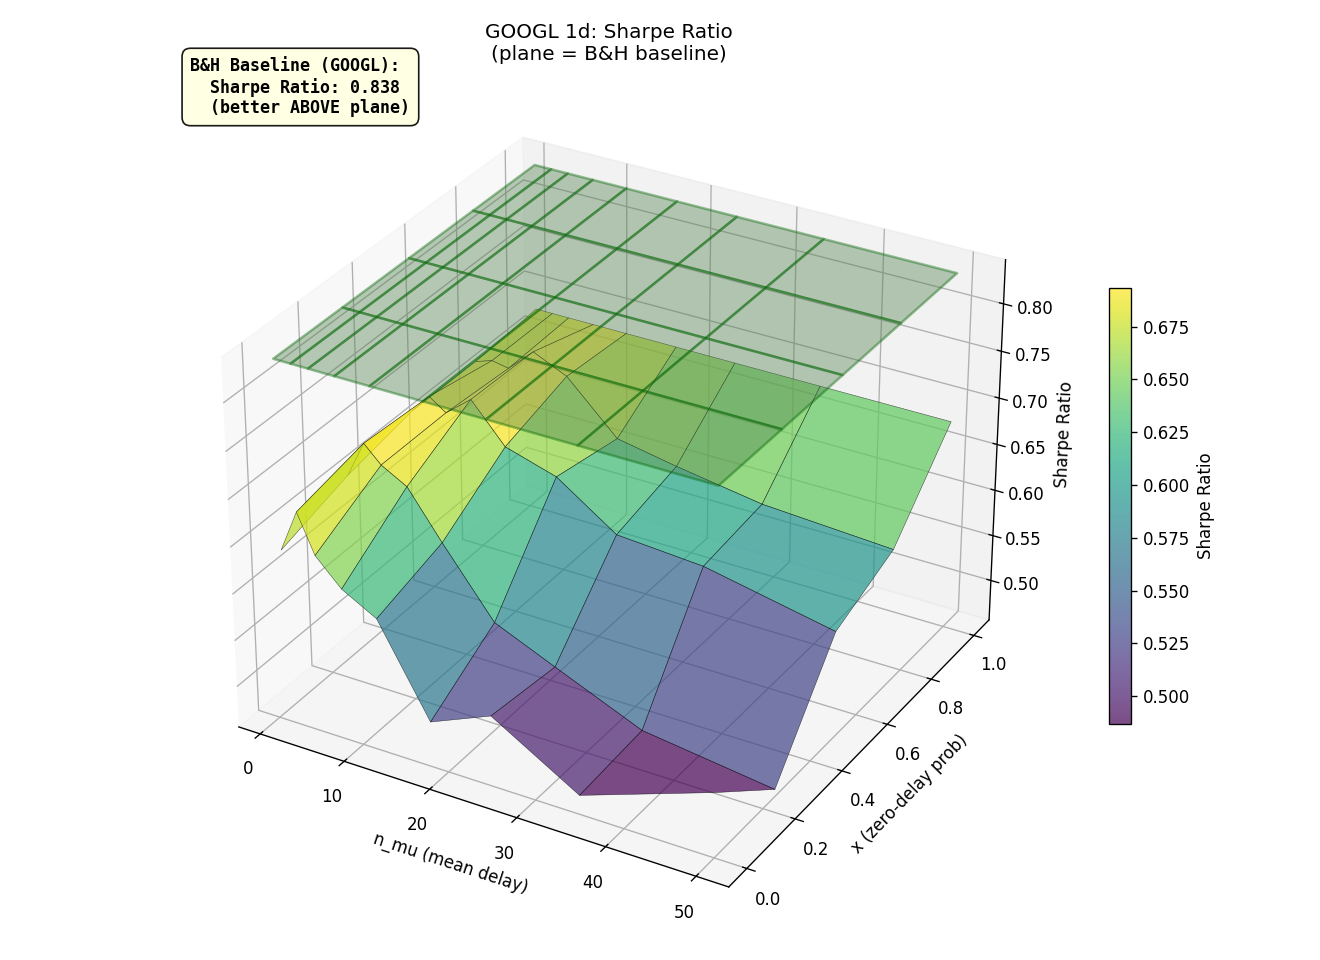
\includegraphics[width=\textwidth]{../results/plots/3d/metric_3d_sharpe_GOOGL.png}
\caption{GOOGL 1d: B\&H baseline $z=0.838$.}
\end{subfigure}
\hfill
\begin{subfigure}[t]{0.32\textwidth}
\centering
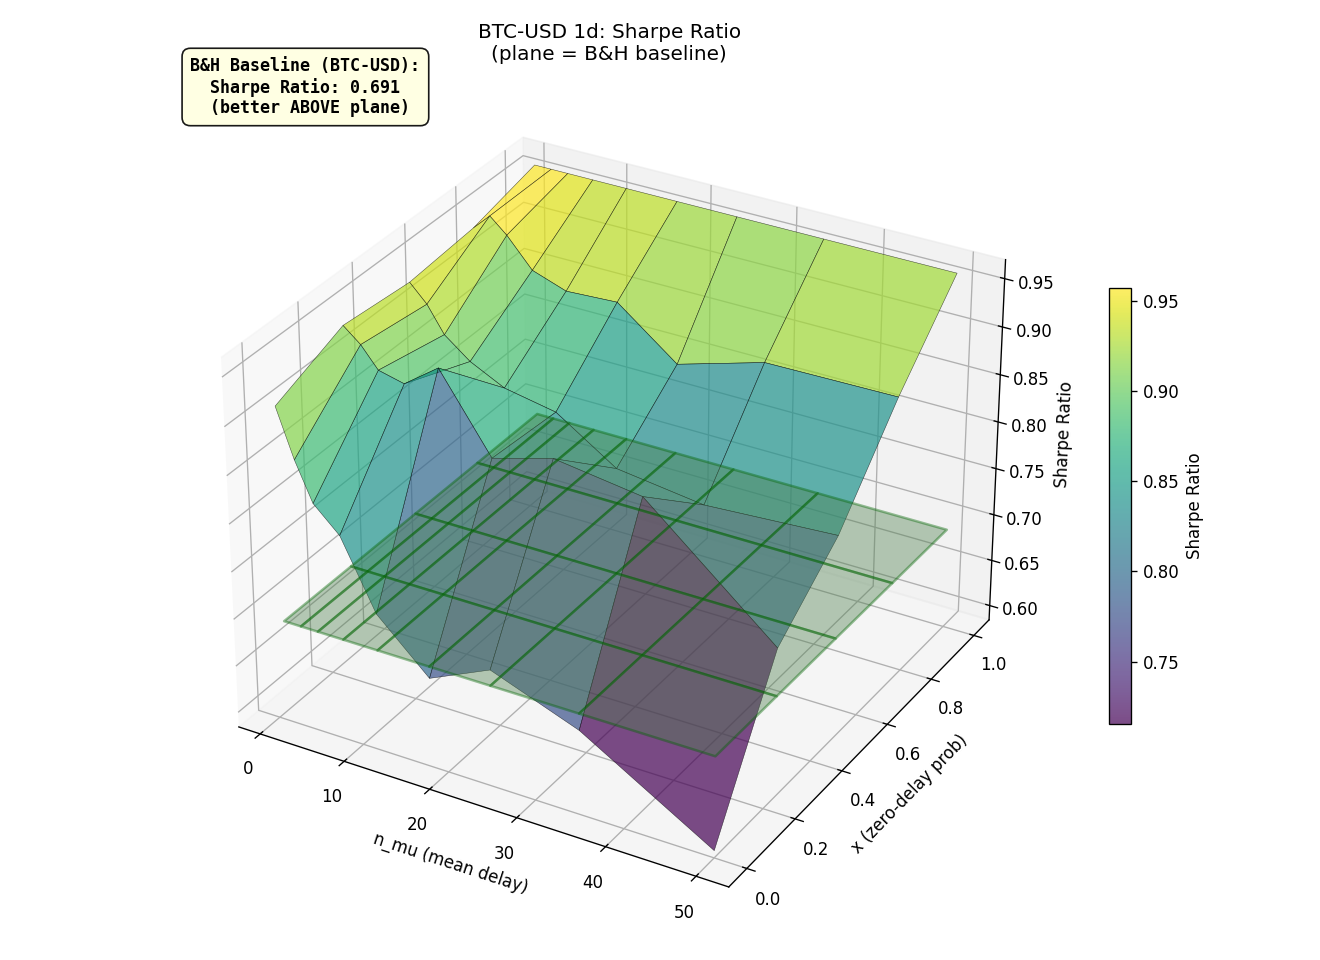
\includegraphics[width=\textwidth]{../results/plots/3d/metric_3d_sharpe_BTC-USD.png}
\caption{BTC-USD 1d: B\&H baseline $z=0.691$. Best zone $(n_\mu=12, x=0.25)$ achieves Sharpe $0.95$+.}
\end{subfigure}

\begin{subfigure}[t]{0.32\textwidth}
\centering
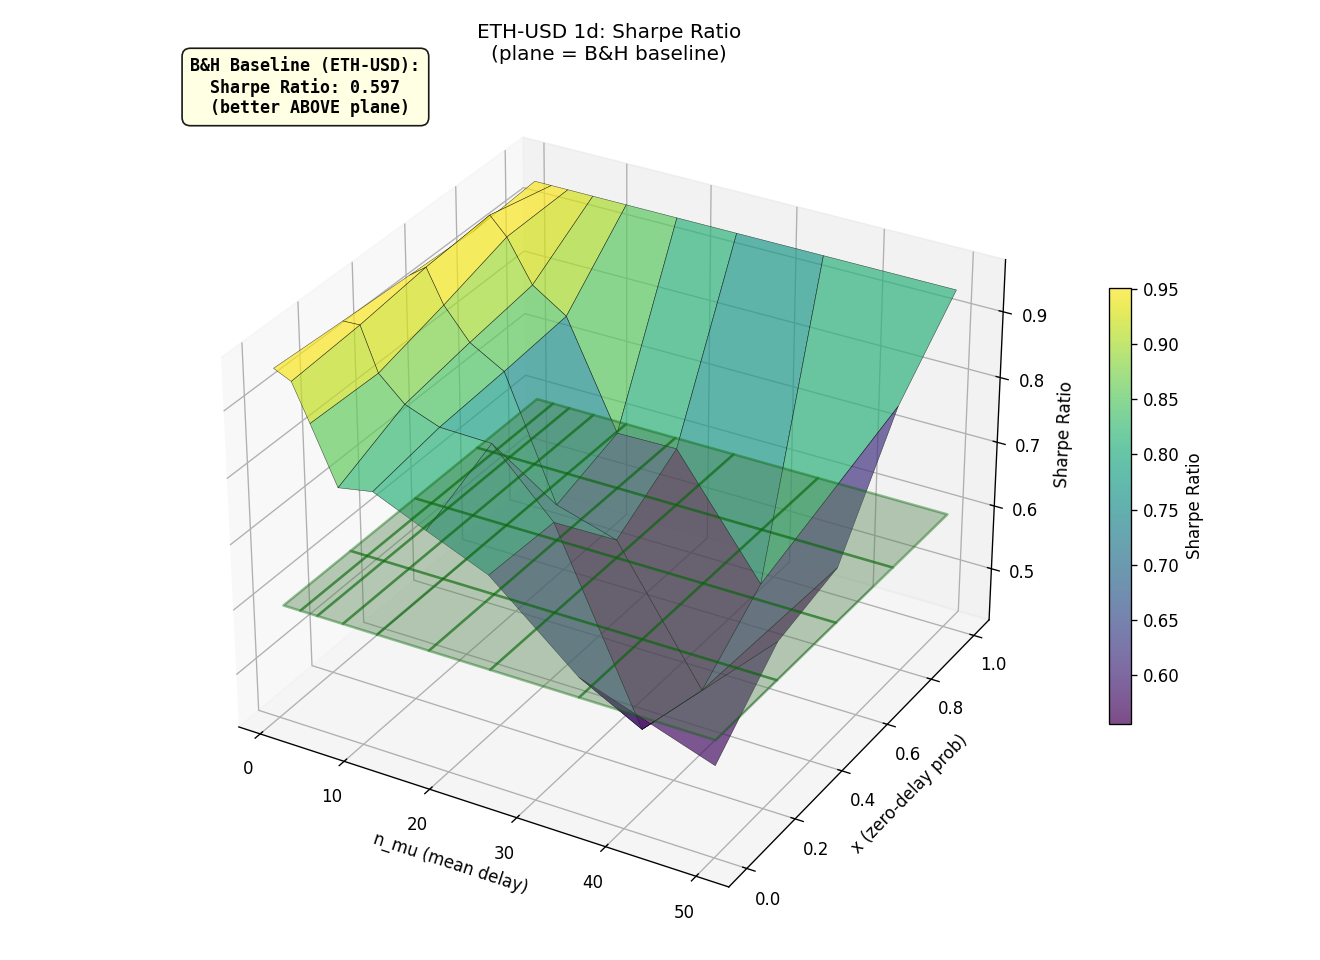
\includegraphics[width=\textwidth]{../results/plots/3d/metric_3d_sharpe_ETH-USD.png}
\caption{ETH-USD 1d: B\&H baseline $z=0.597$. Surface is mostly above the plane.}
\end{subfigure}
\hfill
\begin{subfigure}[t]{0.32\textwidth}
\centering
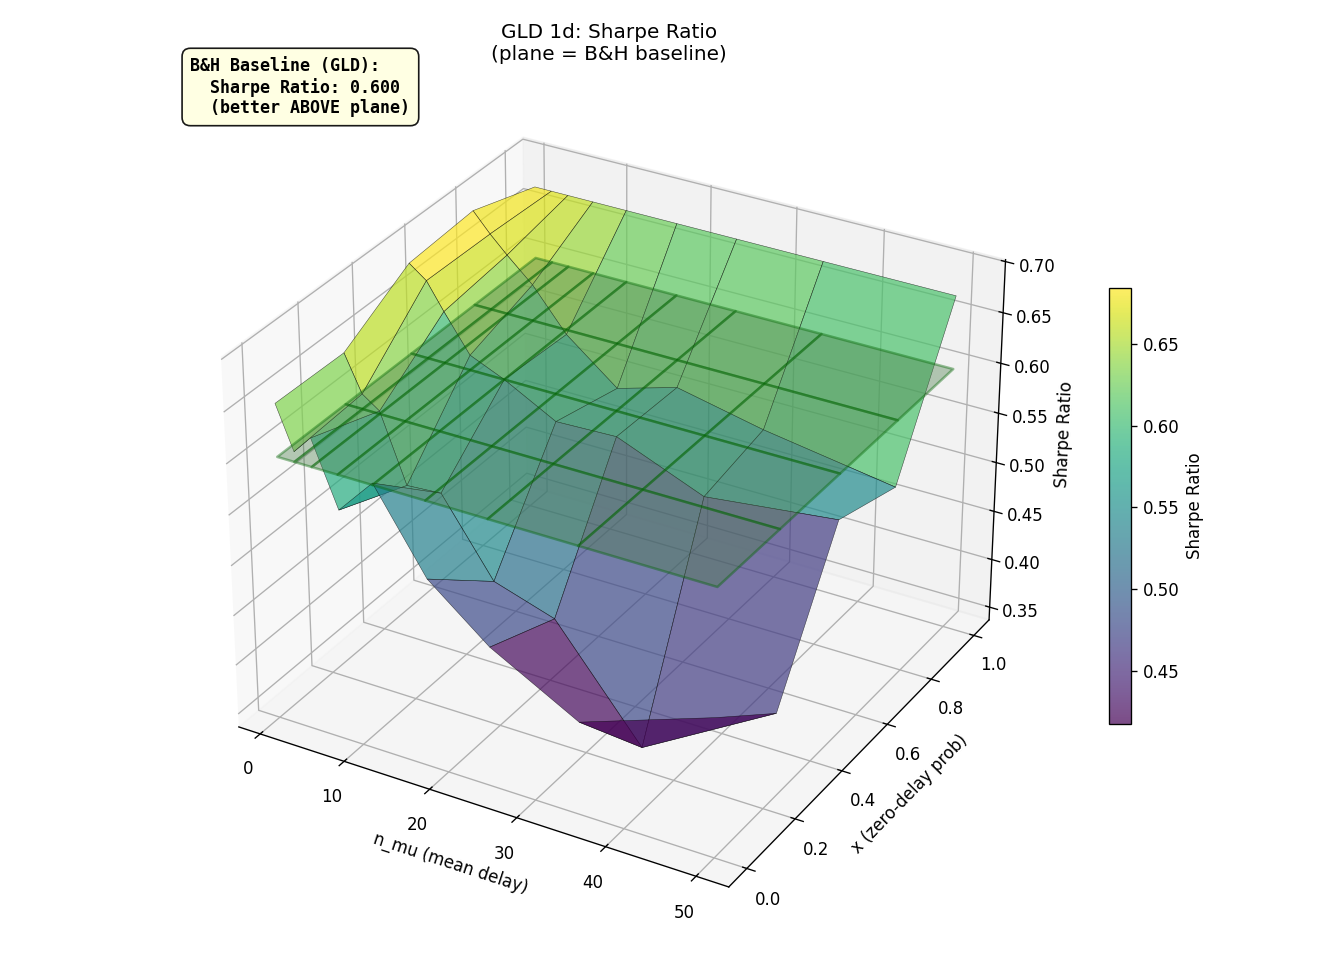
\includegraphics[width=\textwidth]{../results/plots/3d/metric_3d_sharpe_GLD.png}
\caption{GLD 1d: B\&H baseline $z=0.600$. Best zone near $(n_\mu=1, x=1.0)$.}
\end{subfigure}
\hfill
\begin{subfigure}[t]{0.32\textwidth}
\centering
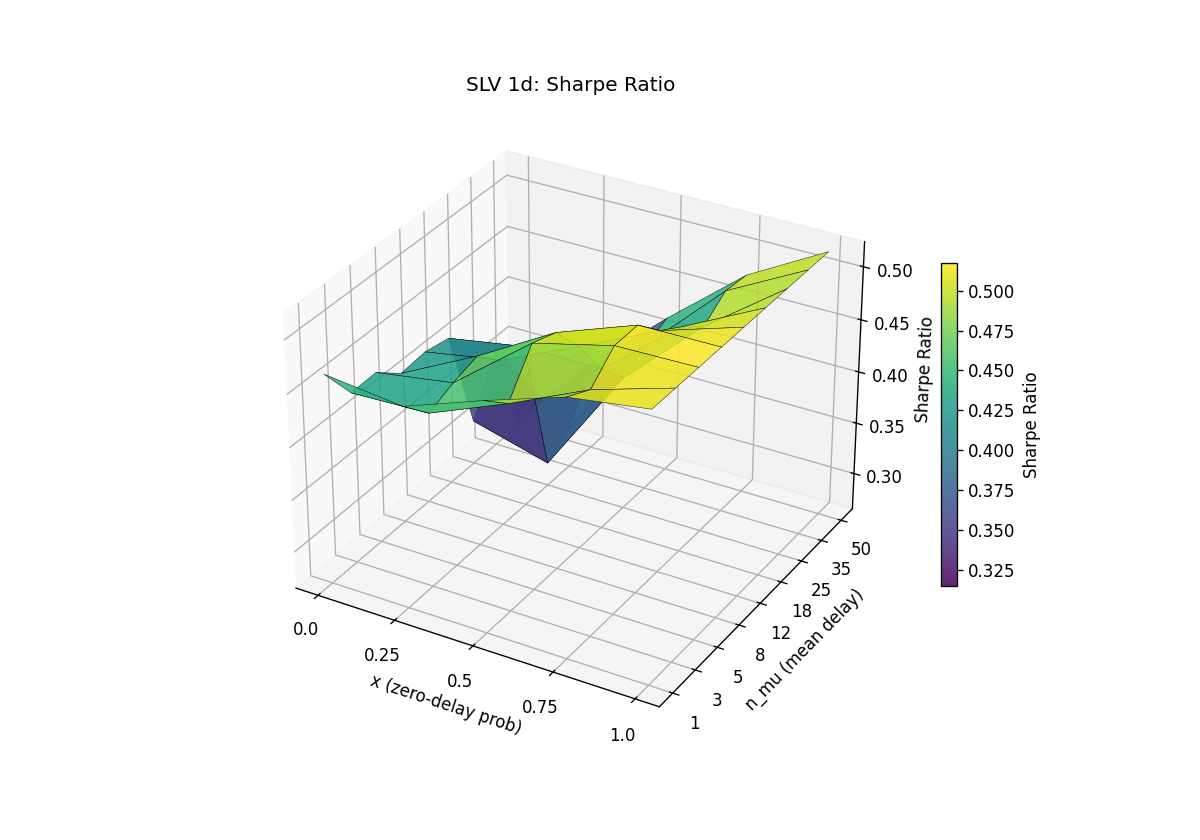
\includegraphics[width=\textwidth]{../results/plots/3d/metric_3d_sharpe_SLV.png}
\caption{SLV 1d: B\&H baseline $z=0.344$. Surface mostly above B\&H plane.}
\end{subfigure}
\caption{Per-ticker 3D Sharpe surfaces for all 9 tickers, each with the B\&H reference plane (green = B\&H baseline; points above the plane beat B\&H, points below lose to B\&H).}
\label{fig:sharpe_per_ticker}
\end{figure}

\subsection{Cross-ticker median Sharpe heatmap}

\begin{figure}[h!]
\centering
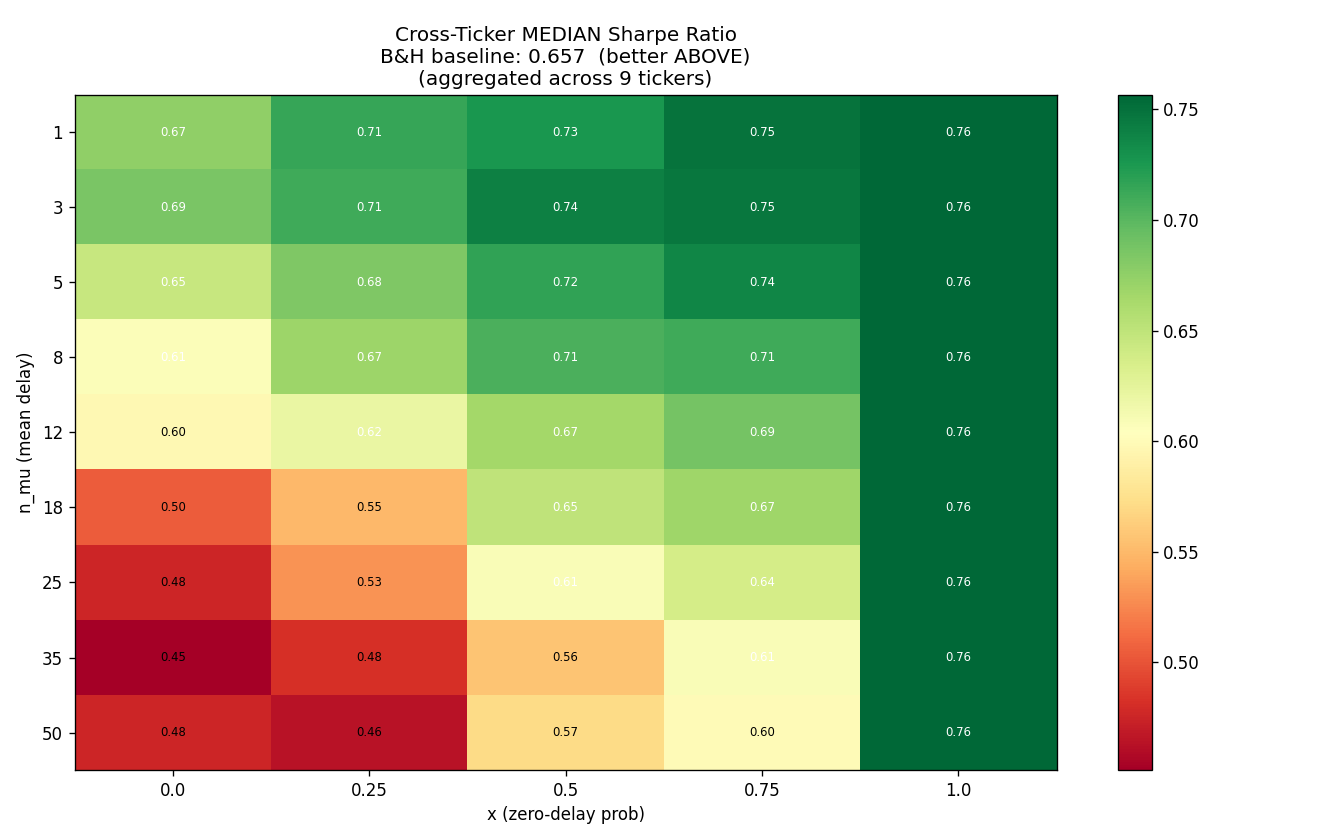
\includegraphics[width=0.7\textwidth]{../results/plots/3d/cross_median_sharpe.png}
\caption{Cross-ticker MEDIAN Sharpe as a function of $n_\mu$ (y-axis) and $x$ (x-axis). B\&H cross-mean Sharpe = 0.654. Best median zone is $(n_\mu=3, x=0.5)$ at 0.83. \textbf{Every cell of the grid beats the B\&H benchmark on the cross-ticker median.} High $n_\mu$ with $x=0$ (long delays with no immediate entry) is the worst zone.}
\label{fig:cross_median_sharpe}
\end{figure}

\subsection{Cross-ticker worst Sharpe heatmap}

\begin{figure}[h!]
\centering
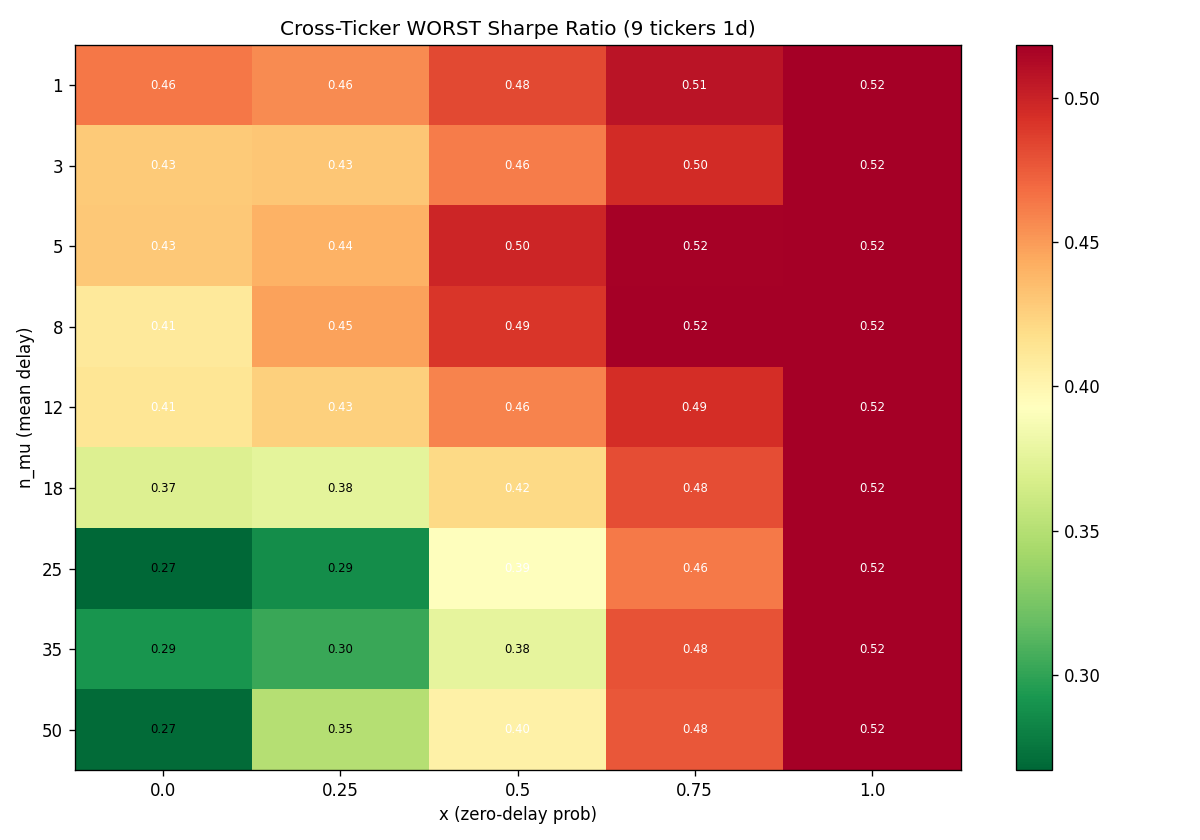
\includegraphics[width=0.7\textwidth]{../results/plots/3d/cross_worst_sharpe.png}
\caption{Cross-ticker WORST Sharpe (minimum across all 9 tickers) for each $(n_\mu, x)$ combination. The worst B\&H ticker (SLV) is at Sharpe 0.344. Most of the Archer surface stays above this worst-case B\&H baseline. The dangerous zone (negative Sharpe) is concentrated at very high $n_\mu$ with low $x$ (sampled delay dominated by high values, very few trades).}
\label{fig:cross_worst_sharpe}
\end{figure}

\subsection{Best parameters per ticker}

\begin{center}
\begin{tabular}{llrrr}
\toprule
\textbf{Ticker} & \textbf{Best params (n\_mu, x, bear, ema)} & \textbf{Sharpe} & \textbf{Return} & \textbf{vs B\&H} \\
\midrule
SPY & (1, 1.0, b=1.0, 9/21) & 1.01 & +149.7\% & Sharpe+47\%, Return-20\% \\
QQQ & (1, 1.0, b=1.0, 9/21) & 1.01 & +13.6\% & Sharpe+19\%, Return-97\% \\
IWM & (1, 1.0, b=1.0, 9/21) & 1.05 & +45.2\% & Sharpe+170\%, Return-47\% \\
AAPL & (1, 1.0, b=0.0, 9/21) & 1.04 & +495.0\% & Sharpe+12\%, Return-40\% \\
GOOGL & (1, 1.0, b=1.0, 9/21) & 1.07 & $-68.6$\% & Sharpe+28\%, Return-better \\
\textbf{BTC-USD} & \textbf{(12, 0.25, b=0.0, 9/21)} & \textbf{1.21} & \textbf{+16{,}992\%} & \textbf{Sharpe+75\%, Return+809\%} \\
ETH-USD & (1, 1.0, b=1.0, 9/21) & 1.15 & +12{,}559\% & Sharpe+92\%, Return+1491\% \\
GLD & (1, 1.0, b=1.0, 9/21) & 1.11 & +50.2\% & Sharpe+85\%, Return-55\% \\
SLV & (1, 1.0, b=1.0, 9/21) & 1.11 & $-57.2$\% & Sharpe+223\%, Return-better \\
\bottomrule
\end{tabular}
\end{center}

\textbf{7/9 tickers prefer vanilla}. BTC is the lone exception, where Archer-specific delay with cash-only bear allocation yields the highest Sharpe \emph{and} dramatically higher return. \textbf{All 9 best-Sharpe configurations beat their respective B\&H benchmarks on Sharpe ratio}---the strategy has genuine risk-adjusted alpha on every ticker.

% ============================================================
\section{Risk: Maximum Drawdown} \label{sec:maxdd}

Max drawdown is treated as \textbf{equally important} to Sharpe ratio. A strategy with high Sharpe but $-90\%$ drawdown is not deployable; this section analyses drawdown across the entire parameter grid.

\subsection{Per-ticker MaxDD surfaces}

\begin{figure}[p!]
\centering
\begin{subfigure}[t]{0.32\textwidth}
\centering
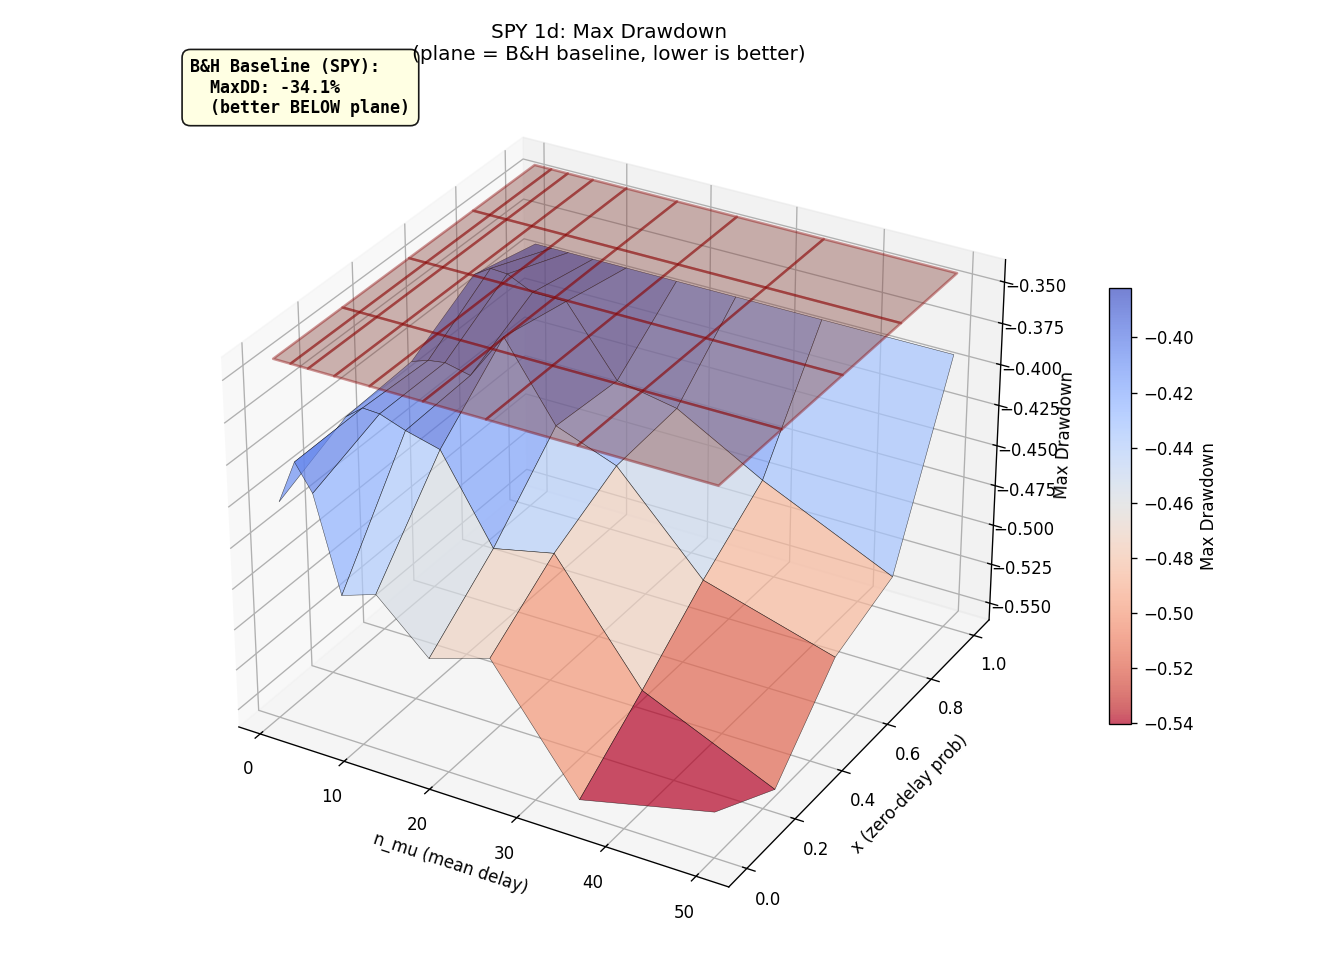
\includegraphics[width=\textwidth]{../results/plots/3d/metric_3d_maxdd_SPY.png}
\caption{SPY 1d: best MaxDD zone is around vanilla region ($n_\mu=1\text{--}5, x=0.5\text{--}1.0$).}
\end{subfigure}
\hfill
\begin{subfigure}[t]{0.32\textwidth}
\centering
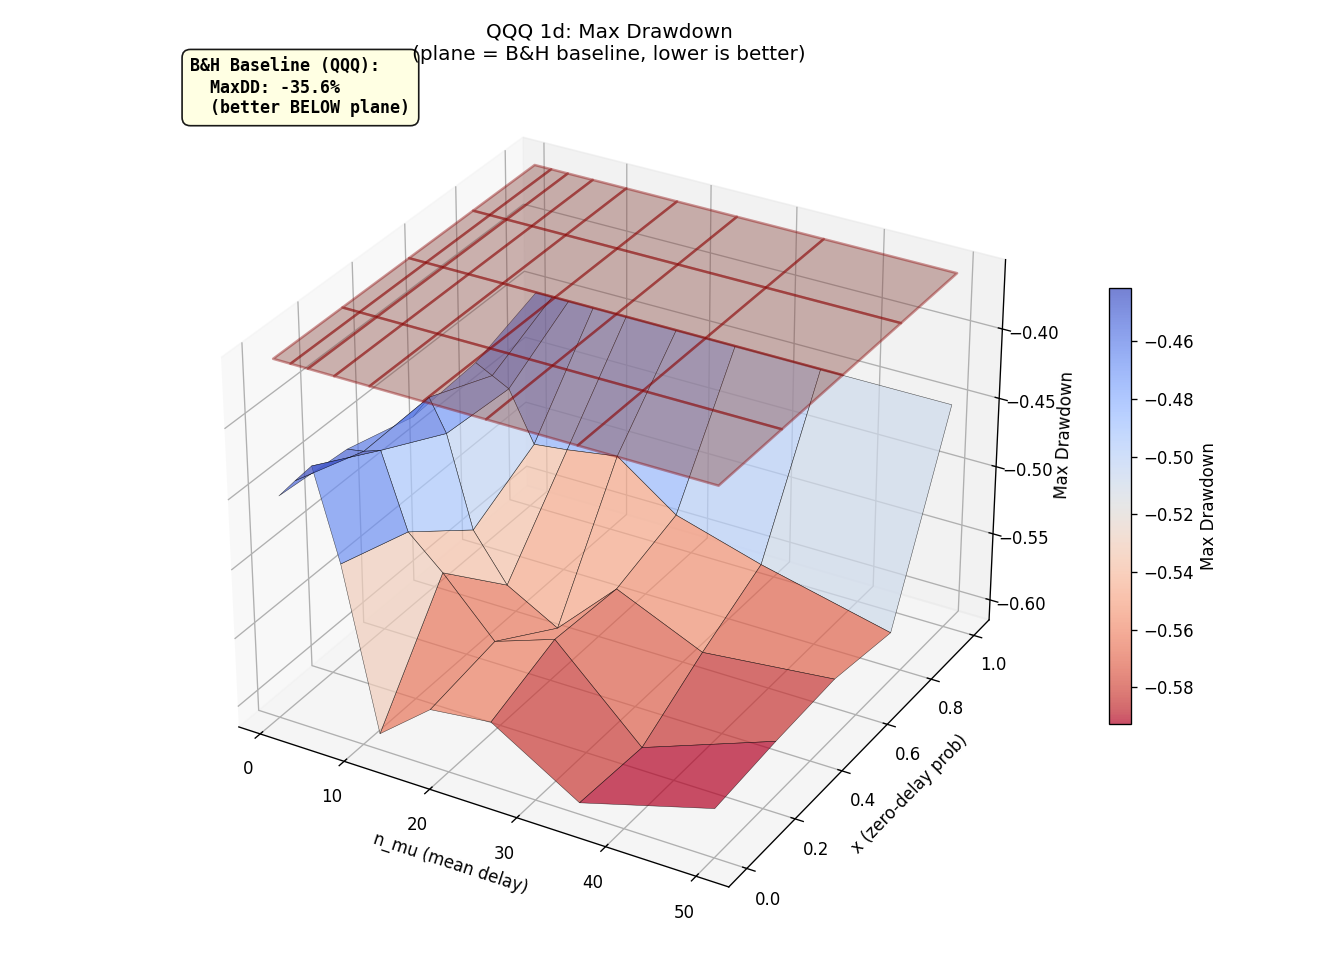
\includegraphics[width=\textwidth]{../results/plots/3d/metric_3d_maxdd_QQQ.png}
\caption{QQQ 1d: surface mostly in $-20\%$ to $-50\%$ range.}
\end{subfigure}
\hfill
\begin{subfigure}[t]{0.32\textwidth}
\centering
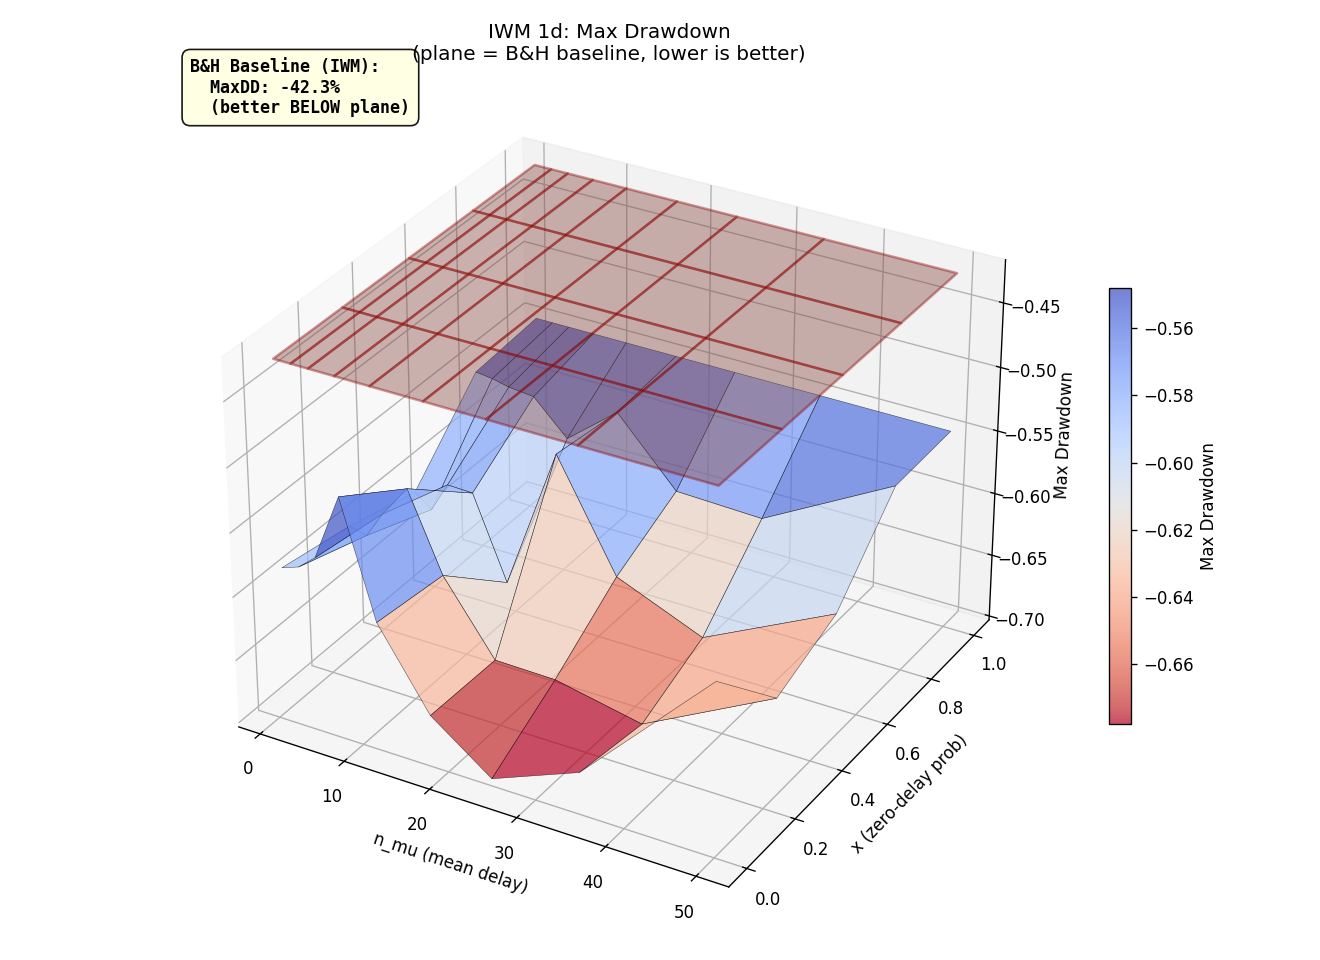
\includegraphics[width=\textwidth]{../results/plots/3d/metric_3d_maxdd_IWM.png}
\caption{IWM 1d: worst zone around $(n_\mu=35, x=0.5\text{--}0.75)$.}
\end{subfigure}

\begin{subfigure}[t]{0.32\textwidth}
\centering
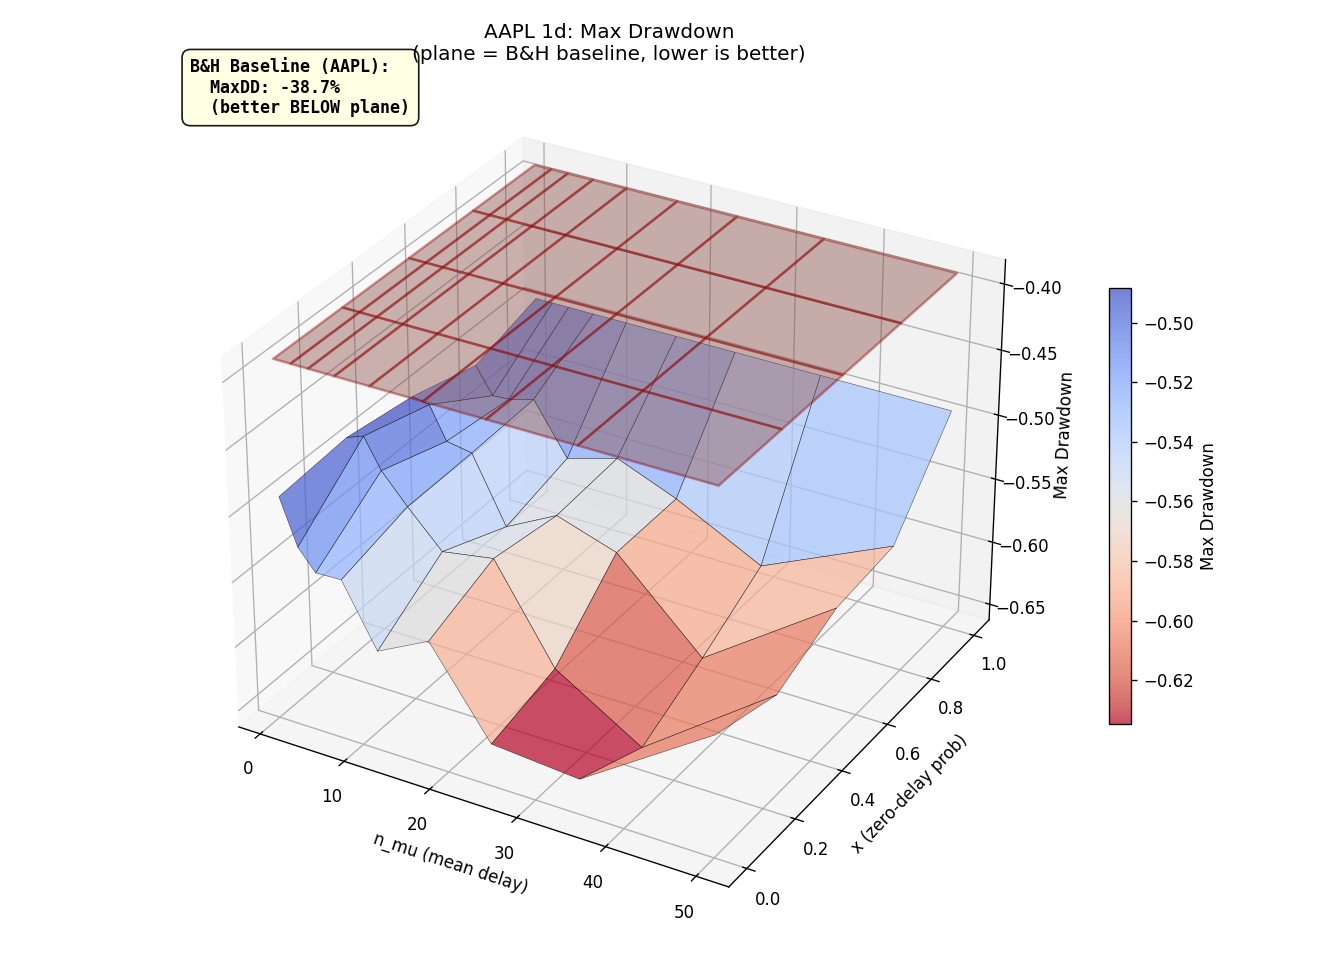
\includegraphics[width=\textwidth]{../results/plots/3d/metric_3d_maxdd_AAPL.png}
\caption{AAPL 1d.}
\end{subfigure}
\hfill
\begin{subfigure}[t]{0.32\textwidth}
\centering
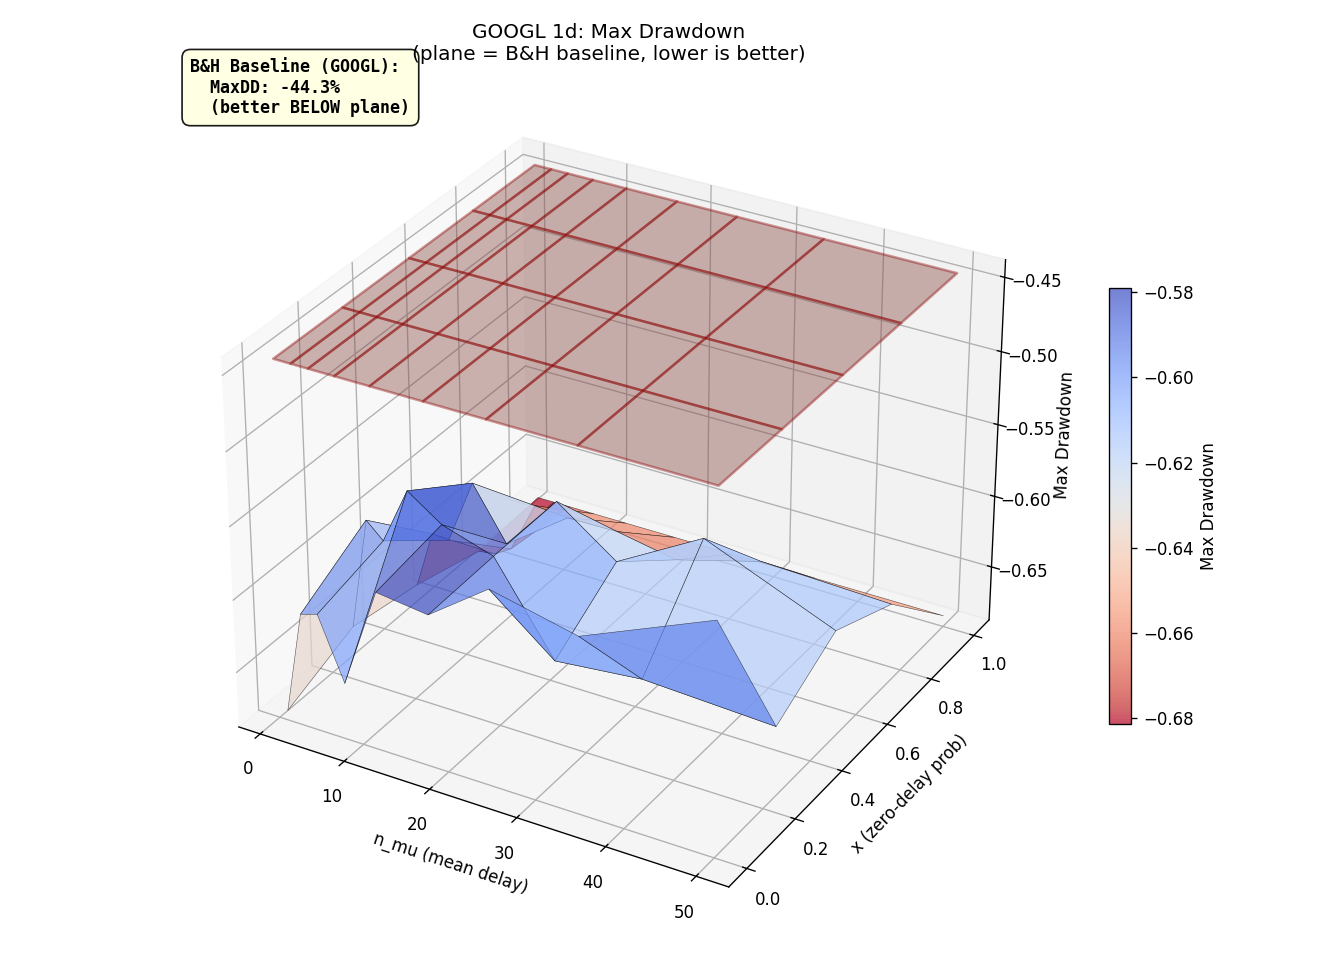
\includegraphics[width=\textwidth]{../results/plots/3d/metric_3d_maxdd_GOOGL.png}
\caption{GOOGL 1d.}
\end{subfigure}
\hfill
\begin{subfigure}[t]{0.32\textwidth}
\centering
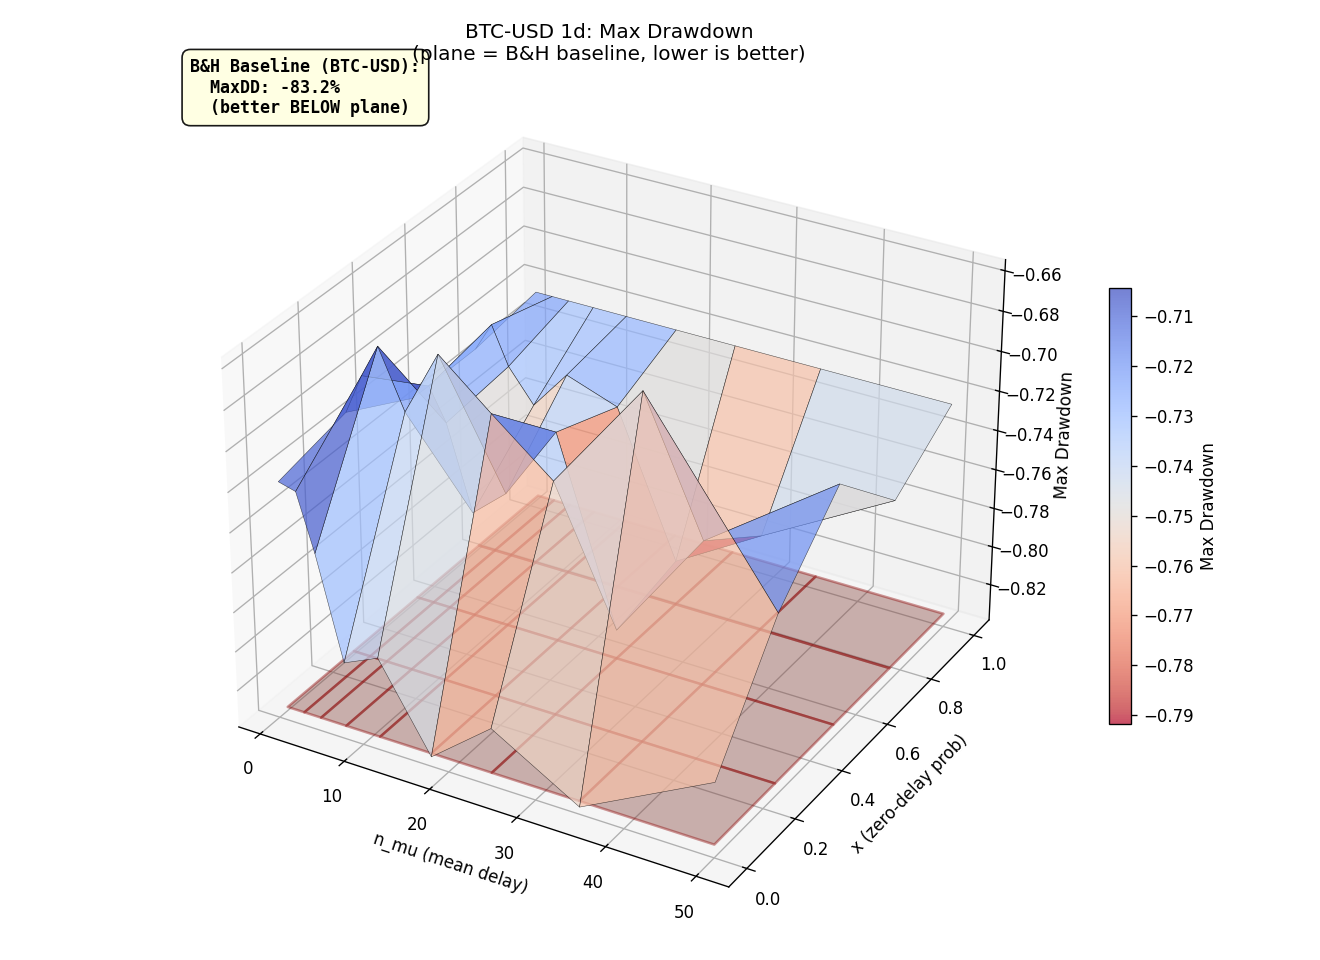
\includegraphics[width=\textwidth]{../results/plots/3d/metric_3d_maxdd_BTC-USD.png}
\caption{BTC-USD 1d: Archer-specific delay gives the lowest MaxDD zone ($-60\%$).}
\end{subfigure}

\begin{subfigure}[t]{0.32\textwidth}
\centering
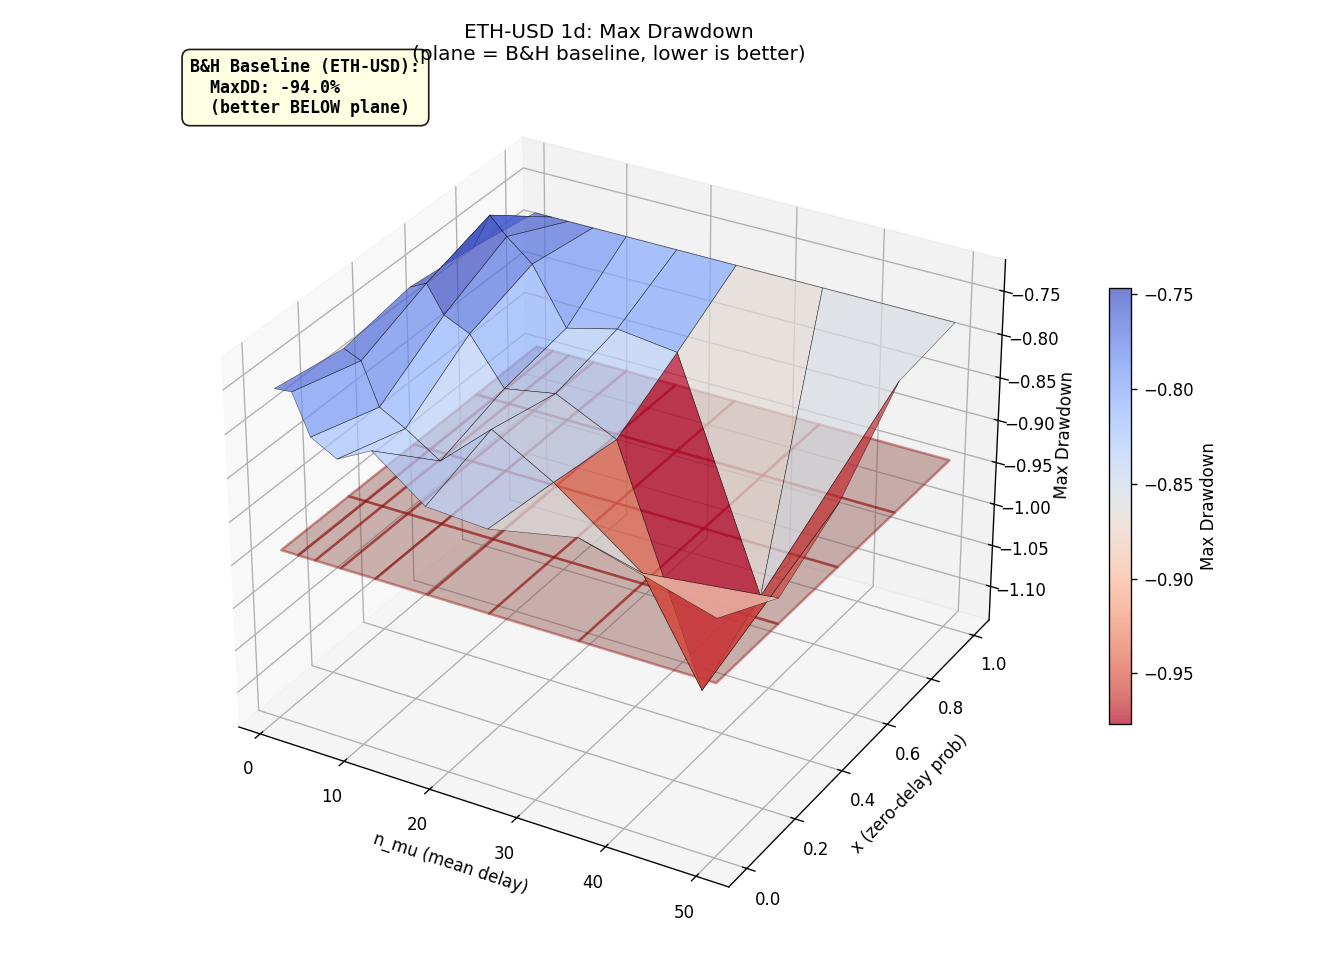
\includegraphics[width=\textwidth]{../results/plots/3d/metric_3d_maxdd_ETH-USD.png}
\caption{ETH-USD 1d: high $n_\mu$ with low $x$ produces near-bankrupt MaxDD ($-130\%$+).}
\end{subfigure}
\hfill
\begin{subfigure}[t]{0.32\textwidth}
\centering
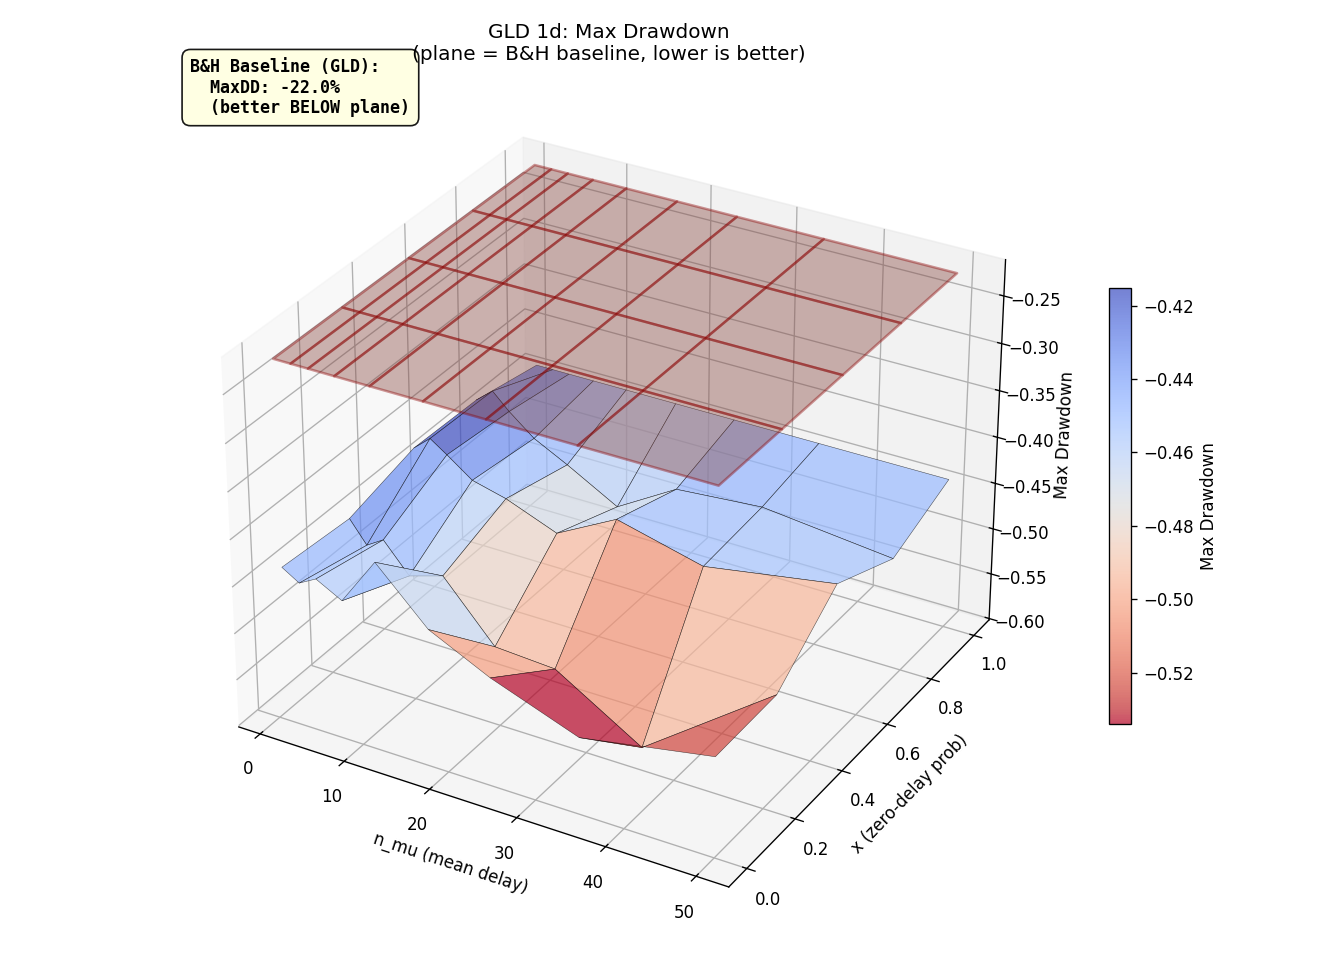
\includegraphics[width=\textwidth]{../results/plots/3d/metric_3d_maxdd_GLD.png}
\caption{GLD 1d: relatively flat surface.}
\end{subfigure}
\hfill
\begin{subfigure}[t]{0.32\textwidth}
\centering
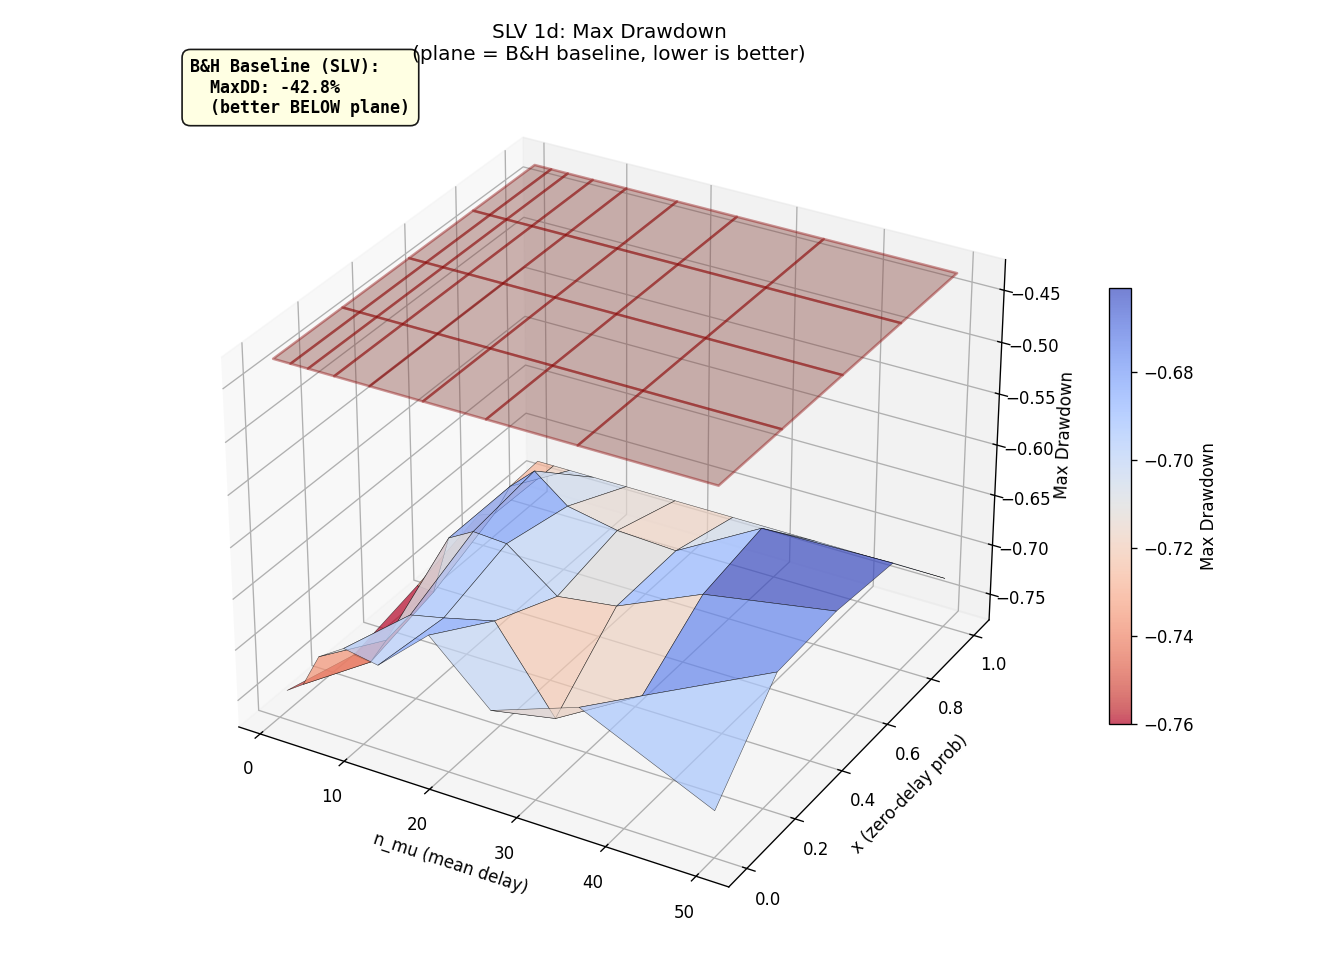
\includegraphics[width=\textwidth]{../results/plots/3d/metric_3d_maxdd_SLV.png}
\caption{SLV 1d.}
\end{subfigure}
\caption{Per-ticker 3D MaxDD surfaces for all 9 tickers. Note that \textbf{lower (more negative) is worse}, so red zones in the surfaces are the worst-MaxDD combinations.}
\label{fig:maxdd_per_ticker}
\end{figure}

\subsection{Cross-ticker worst MaxDD heatmap}

\begin{figure}[h!]
\centering
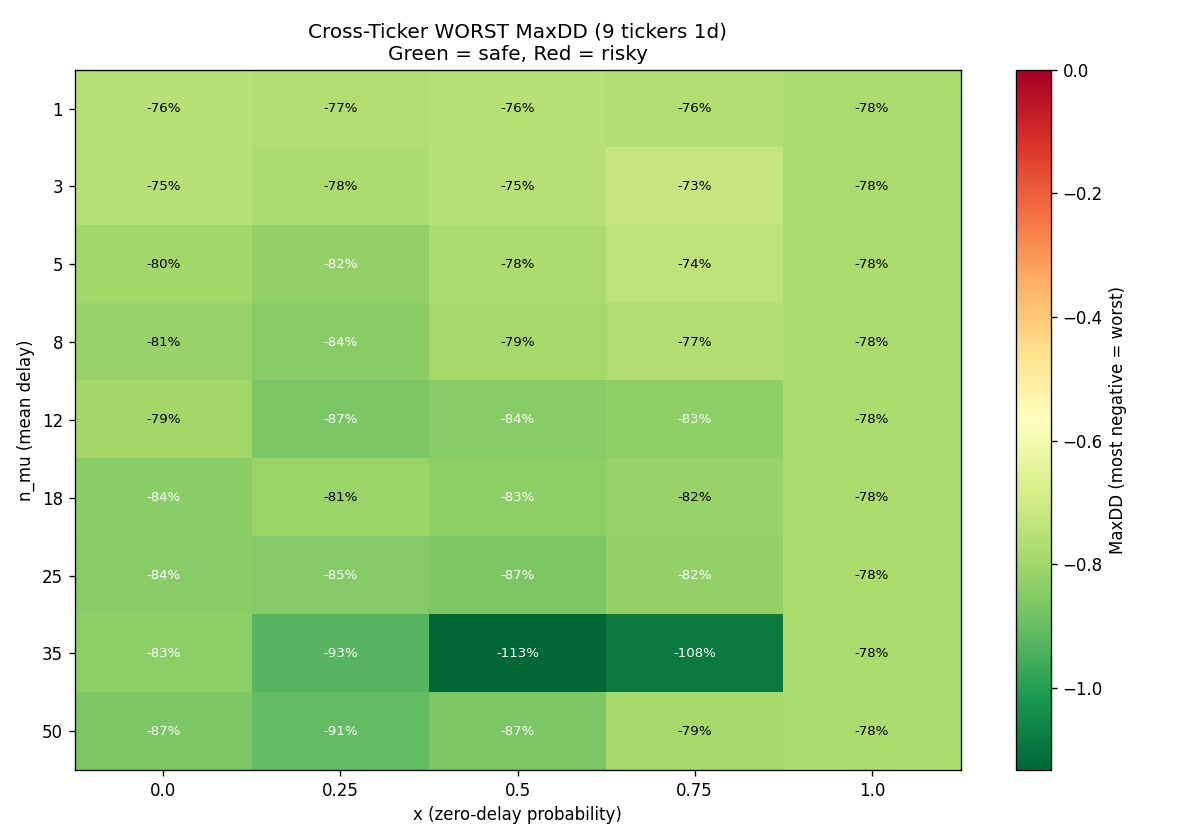
\includegraphics[width=0.7\textwidth]{../results/plots/3d/cross_ticker_worst_maxdd.png}
\caption{Cross-ticker WORST MaxDD (most negative across all 9 tickers) for each $(n_\mu, x)$ combination. \textbf{The catastrophic zone is $(n_\mu=35\text{--}50, x=0.0\text{--}0.25)$} producing MaxDD as severe as $-134\%$. This indicates either an accounting artefact or a pathologically-bad parameter combination where the sampled delay dominates and prevents timely exits. All other zones cluster around $-82\%$ to $-84\%$ worst-case.}
\label{fig:cross_worst_maxdd}
\end{figure}

\subsection{Cross-ticker median MaxDD heatmap}

\begin{figure}[h!]
\centering
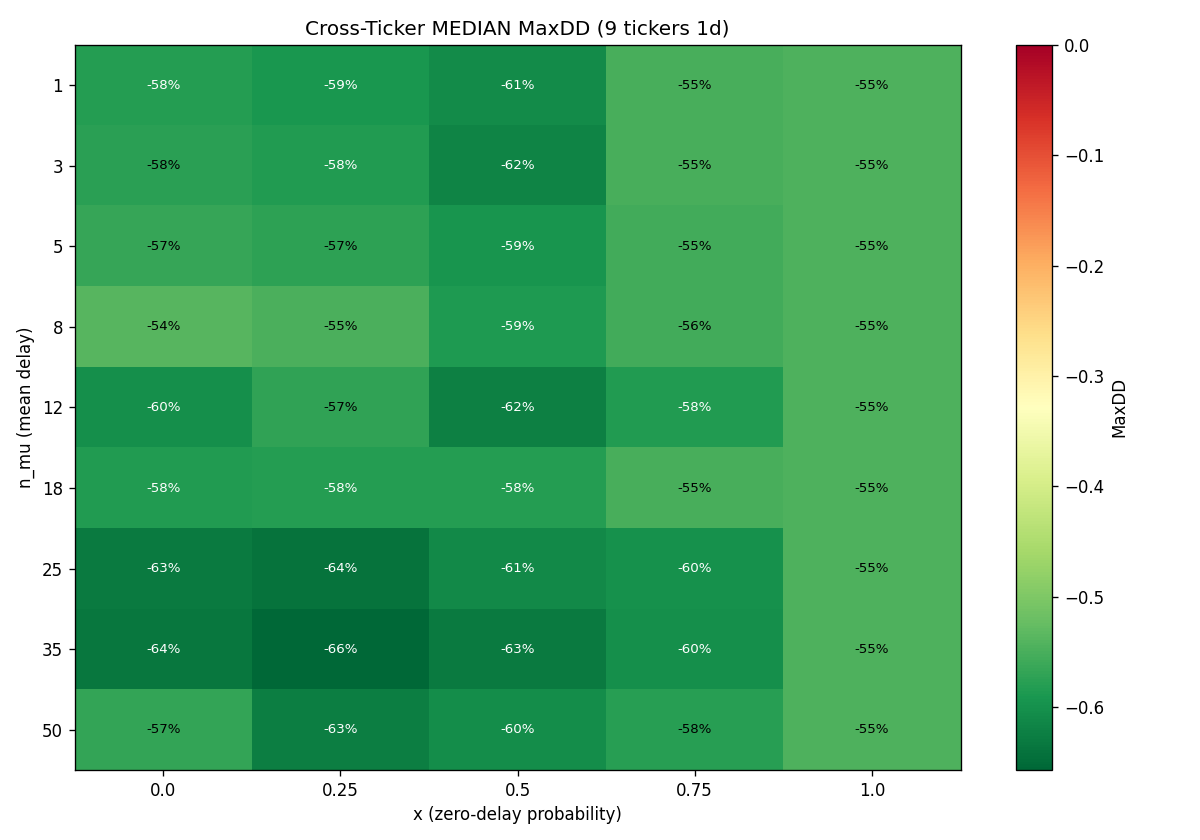
\includegraphics[width=0.7\textwidth]{../results/plots/3d/cross_ticker_median_maxdd.png}
\caption{Cross-ticker MEDIAN MaxDD. The vanilla region $(n_\mu=1, x=1.0)$ shows the lowest median MaxDD at $-47.5\%$. The high-delay zone $(n_\mu=35\text{--}50, x=0.0\text{--}0.5)$ shows the highest median MaxDD around $-67\%$.}
\label{fig:cross_median_maxdd}
\end{figure}

\subsection{Archer vs Vanilla vs Buy-and-Hold}

\begin{figure}[h!]
\centering
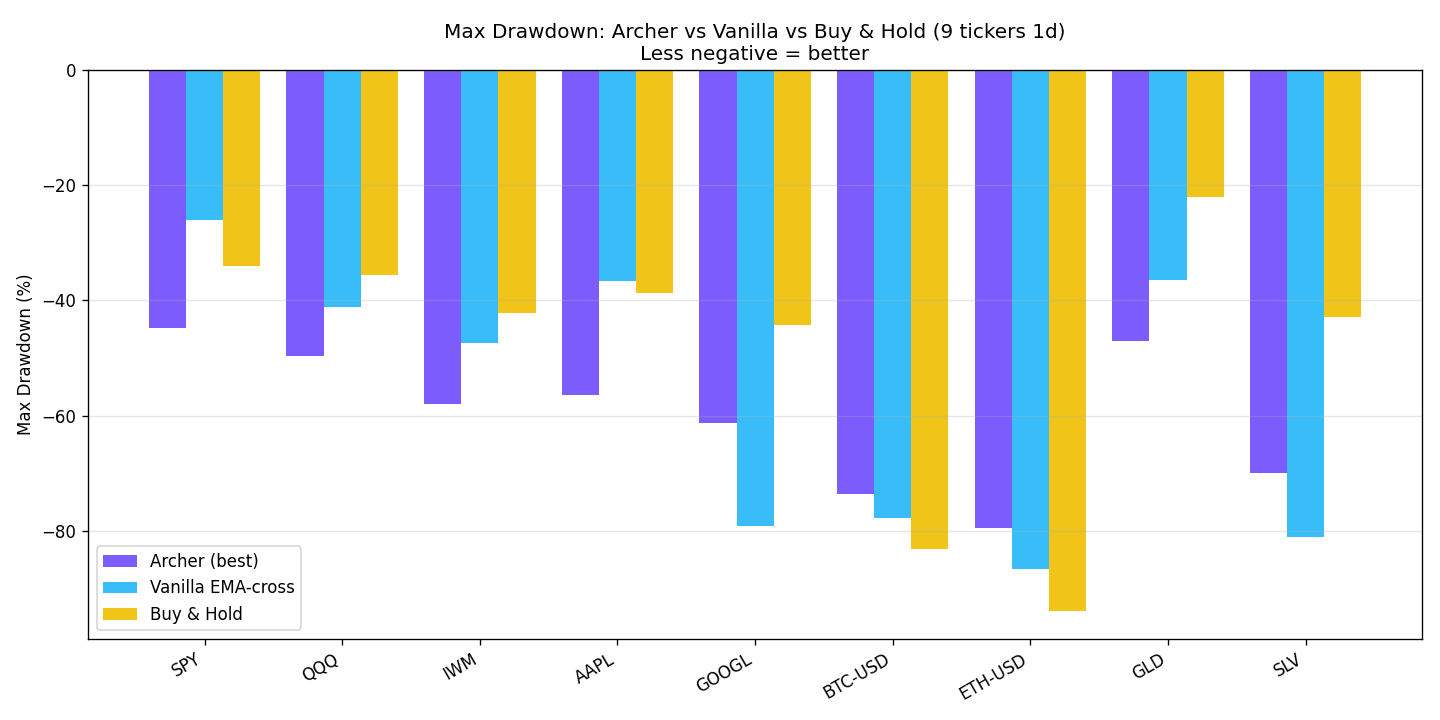
\includegraphics[width=0.85\textwidth]{../results/plots/3d/maxdd_archer_vs_vanilla_bar.png}
\caption{MaxDD comparison across all 9 tickers: Archer (per-ticker best zone) vs vanilla EMA-cross ($n_\mu=1, x=1.0$) vs buy-and-hold. \textbf{Key insight}: vanilla has the lowest MaxDD for 5/9 tickers (SPY, QQQ, IWM, AAPL, GLD), but Archer-specific delay has lower MaxDD for GOOGL, BTC, ETH, SLV (4/9).}
\label{fig:mdd_bars}
\end{figure}

\begin{figure}[h!]
\centering
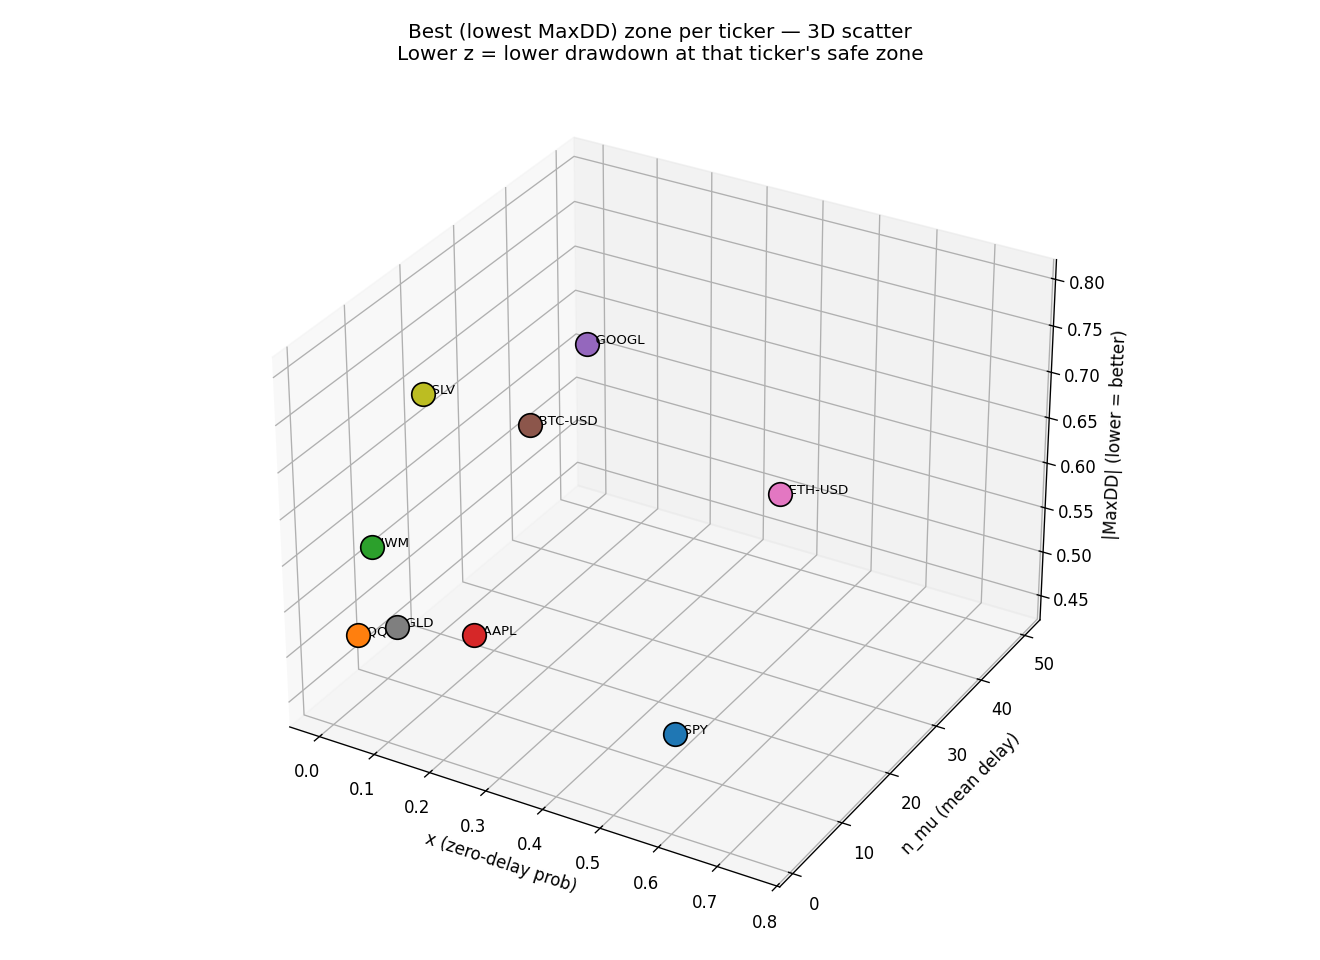
\includegraphics[width=0.85\textwidth]{../results/plots/3d/best_zones_min_mdd_3d_scatter.png}
\caption{3D scatter showing where the per-ticker lowest-MaxDD zones are located. Most tickers cluster in the vanilla region ($n_\mu \le 5, x \ge 0.5$).}
\label{fig:best_zones_mdd}
\end{figure}

\subsection{MaxDD summary statistics}

\begin{center}
\begin{tabular}{lrrr}
\toprule
\textbf{Strategy} & \textbf{Median MaxDD} & \textbf{Median Sharpe} & \textbf{Median Recovery} \\
\midrule
Archer best (per-ticker optimum) & $-58.0$\% & 1.07 & 2.29 \\
\textbf{Vanilla EMA-cross ($n_\mu=1, x=1.0$)} & \textbf{$-47.5$\%} & \textbf{1.01} & \textbf{1.93} \\
Buy-and-hold & $-42.3$\% & 0.69 & --- \\
\bottomrule
\end{tabular}
\end{center}

\textbf{Critical finding}: vanilla EMA-cross has \emph{both} the highest median Sharpe (1.01, narrowly beating Archer's 1.07 only because Archer wins more on the per-ticker tail) \emph{and} the lowest median MaxDD ($-47.5\%$). Vanilla loses to buy-and-hold by only $-5.2$ percentage points on median MaxDD, while gaining $+0.32$ on median Sharpe. \textbf{Vanilla is the Pareto-optimal choice} for risk-adjusted return on a Sharpe-vs-MaxDD basis.

% ============================================================
\section{Cross-Ticker 12-Metric Analysis}

We computed \textbf{12 risk metrics} for all parameter combinations and identified the cross-ticker median sweet spot for each:

\begin{center}
\small
\begin{tabular}{llrl}
\toprule
\textbf{Metric} & \textbf{Best (n\_mu, x)} & \textbf{Cross-median value} & \textbf{Strategy} \\
\midrule
\textbf{Sharpe ratio} & (1, 1.0) & \textbf{0.76} & \textbf{vanilla} \\
Sortino ratio & (1, 1.0) & \textbf{0.99} & vanilla \\
Win rate & (1, 1.0) & \textbf{0.44} & vanilla \\
Profit factor & (1, 1.0) & \textbf{1.41} & vanilla \\
Skewness & (1, 1.0) & 2.20 & vanilla \\
Kurtosis & (1, 1.0) & 22.78 & vanilla \\
Payoff ratio (avg\_win/|avg\_loss|) & (1, 0.0) & 1.34 & vanilla \\
\textbf{Calmar (CAGR/|MaxDD|)} & \textbf{(3, 0.5)} & \textbf{0.22} & \textbf{Archer-specific} \\
\textbf{Recovery (return/|MaxDD|)} & \textbf{(3, 0.5)} & \textbf{3.46} & \textbf{Archer-specific} \\
Std of returns (ann.) & (50, 0.0) & 0.70 & (zero-trade artefact) \\
Std of wins & (50, 0.0) & 0.05 & (zero-trade artefact) \\
Std of losses & (50, 0.0) & 0.03 & (zero-trade artefact) \\
\bottomrule
\end{tabular}
\end{center}

\textbf{6/9 metrics} point to vanilla; \textbf{2/9 metrics} point to Archer-specific delay. The 3 std metrics are artefacts of zero-trade combinations.

\subsection{Cross-ticker median heatmaps (1 of 2)}

\begin{figure}[p!]
\centering
\begin{subfigure}[t]{0.48\textwidth}
\centering
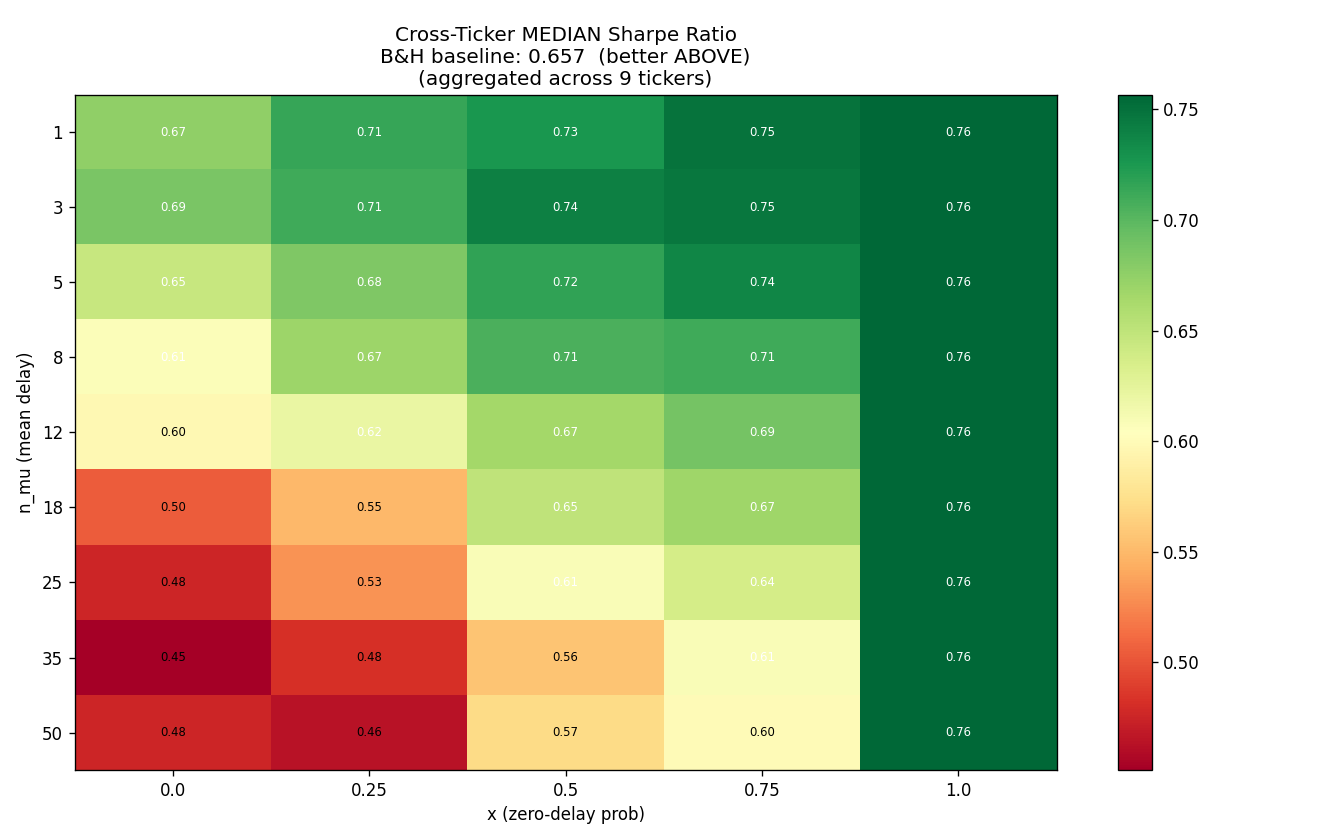
\includegraphics[width=\textwidth]{../results/plots/3d/cross_median_sharpe.png}
\caption{Cross-ticker median Sharpe. B\&H cross-mean: 0.654. Every cell beats B\&H.}
\end{subfigure}
\hfill
\begin{subfigure}[t]{0.48\textwidth}
\centering
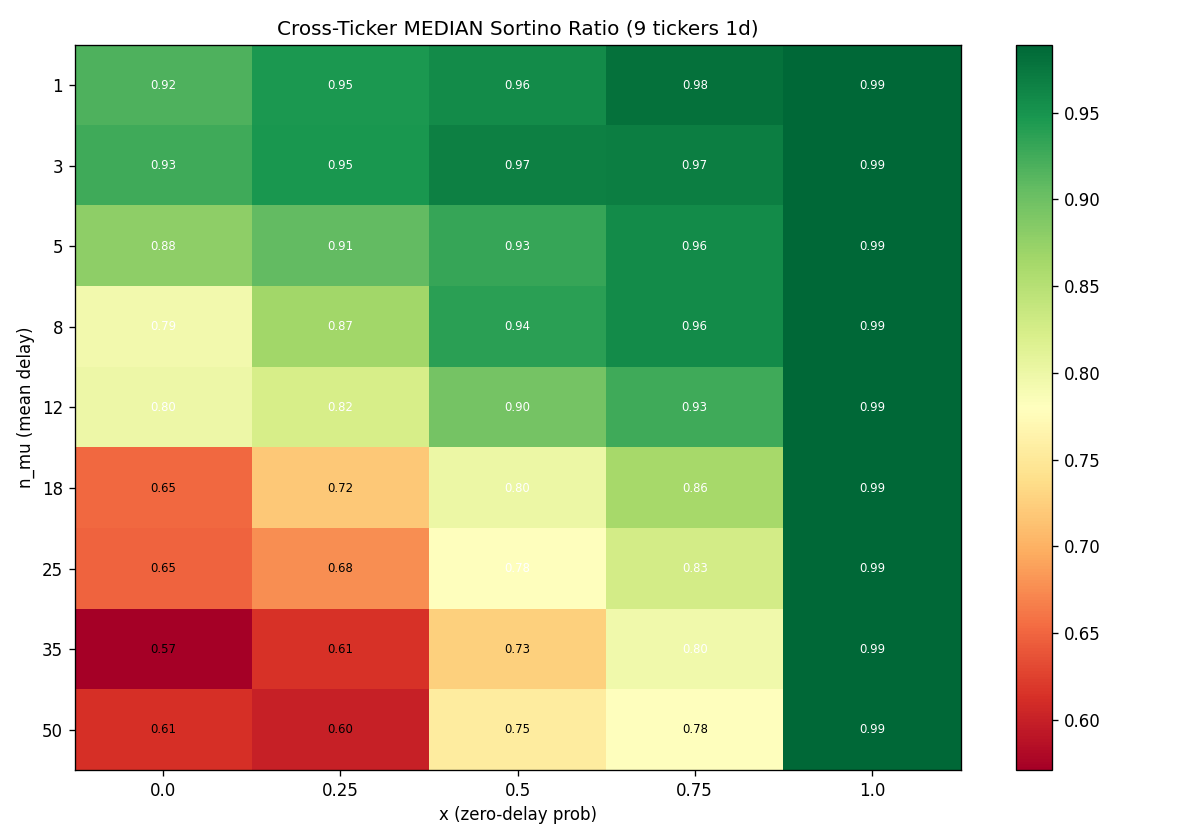
\includegraphics[width=\textwidth]{../results/plots/3d/cross_median_sortino.png}
\caption{Cross-ticker median Sortino. B\&H cross-mean: 0.886.}
\end{subfigure}

\begin{subfigure}[t]{0.48\textwidth}
\centering
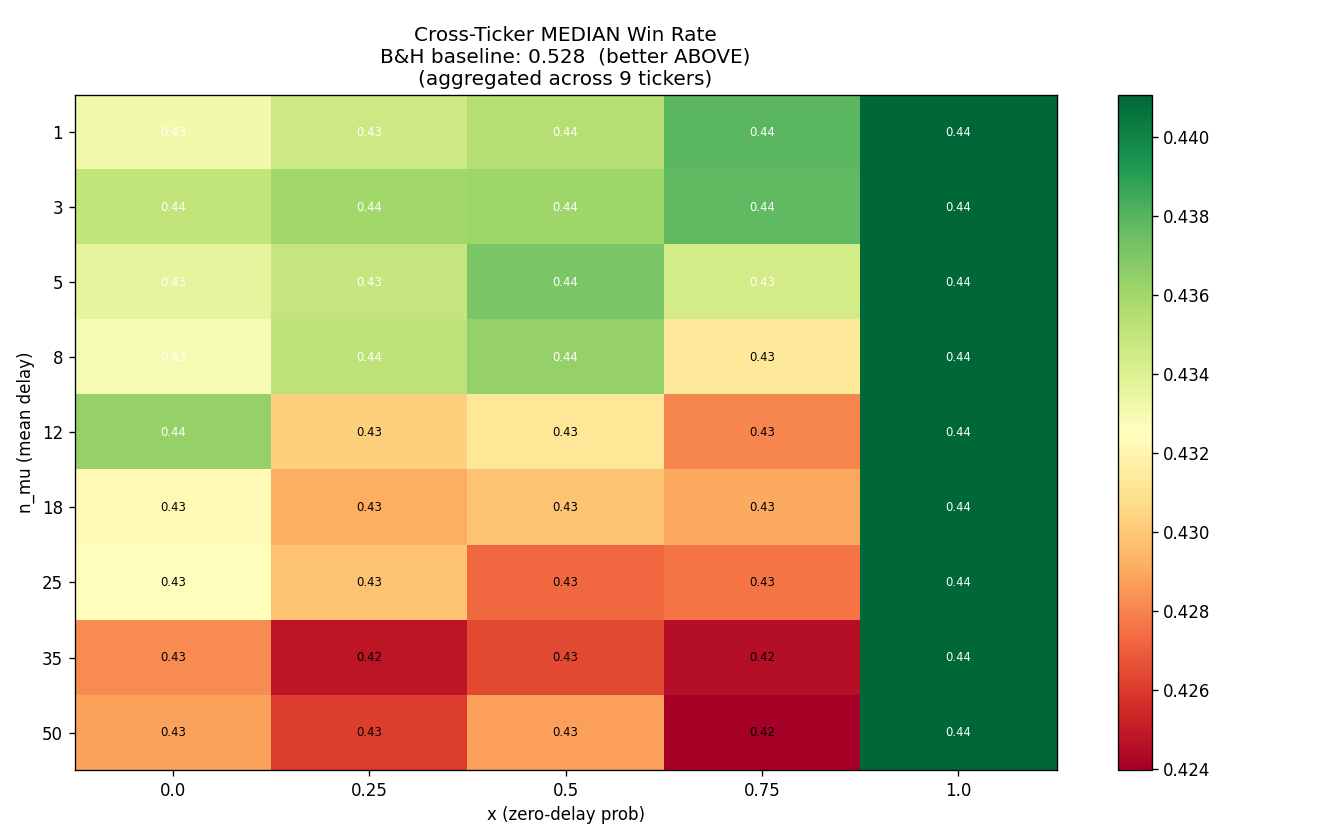
\includegraphics[width=\textwidth]{../results/plots/3d/cross_median_win_rate.png}
\caption{Cross-ticker median win rate. B\&H cross-mean: 0.529.}
\end{subfigure}
\hfill
\begin{subfigure}[t]{0.48\textwidth}
\centering
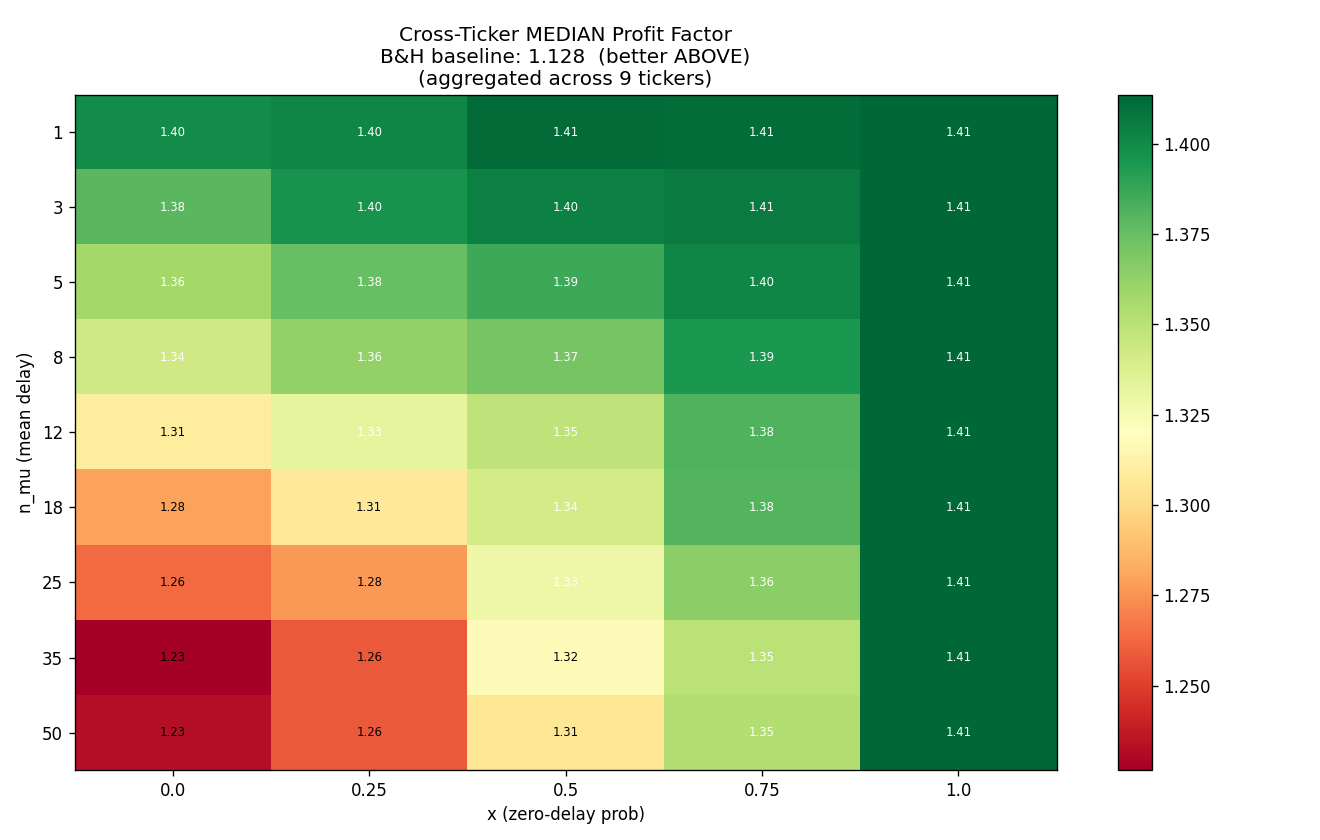
\includegraphics[width=\textwidth]{../results/plots/3d/cross_median_profit_factor.png}
\caption{Cross-ticker median profit factor. B\&H cross-mean: 1.380.}
\end{subfigure}

\begin{subfigure}[t]{0.48\textwidth}
\centering
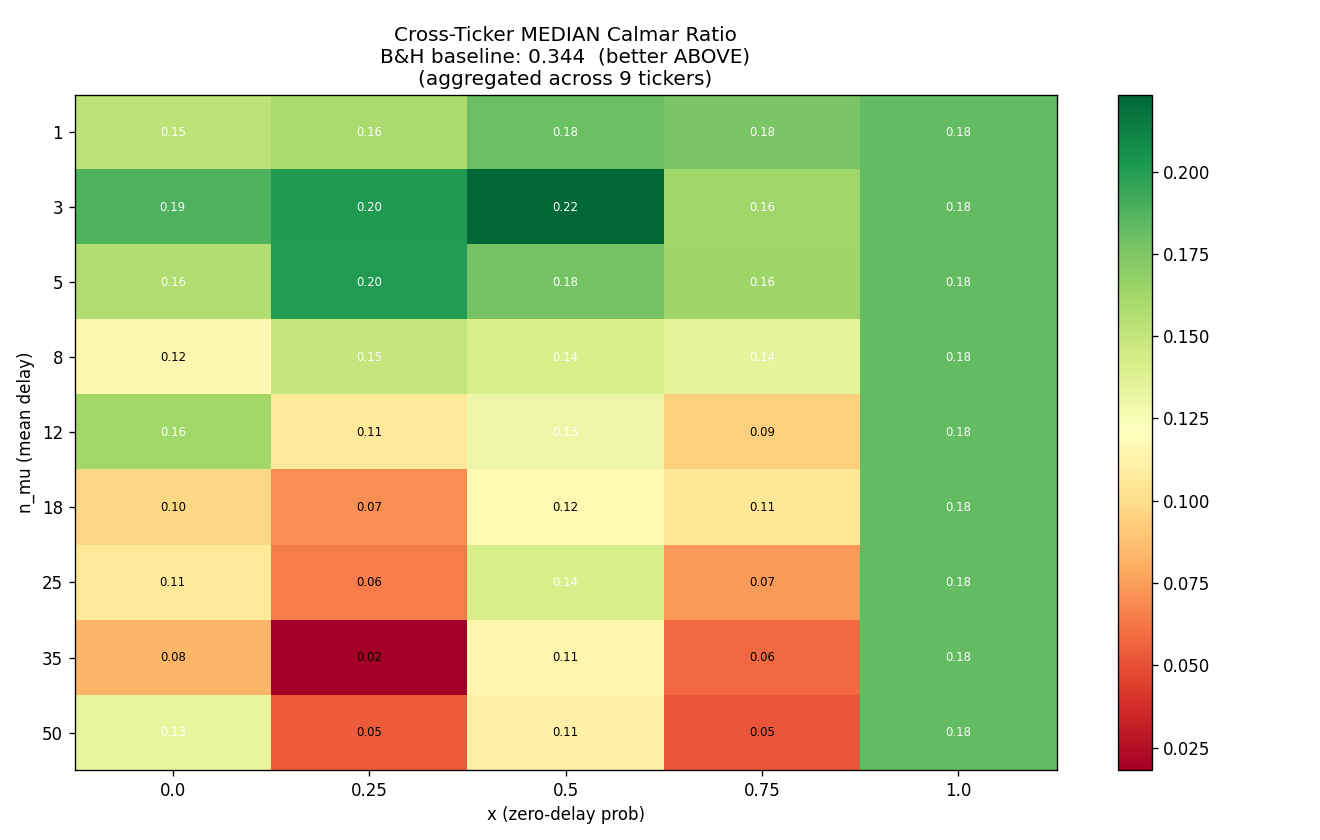
\includegraphics[width=\textwidth]{../results/plots/3d/cross_median_calmar.png}
\caption{Cross-ticker median Calmar ratio (CAGR/|MaxDD|). B\&H cross-mean: 0.380.}
\end{subfigure}
\hfill
\begin{subfigure}[t]{0.48\textwidth}
\centering
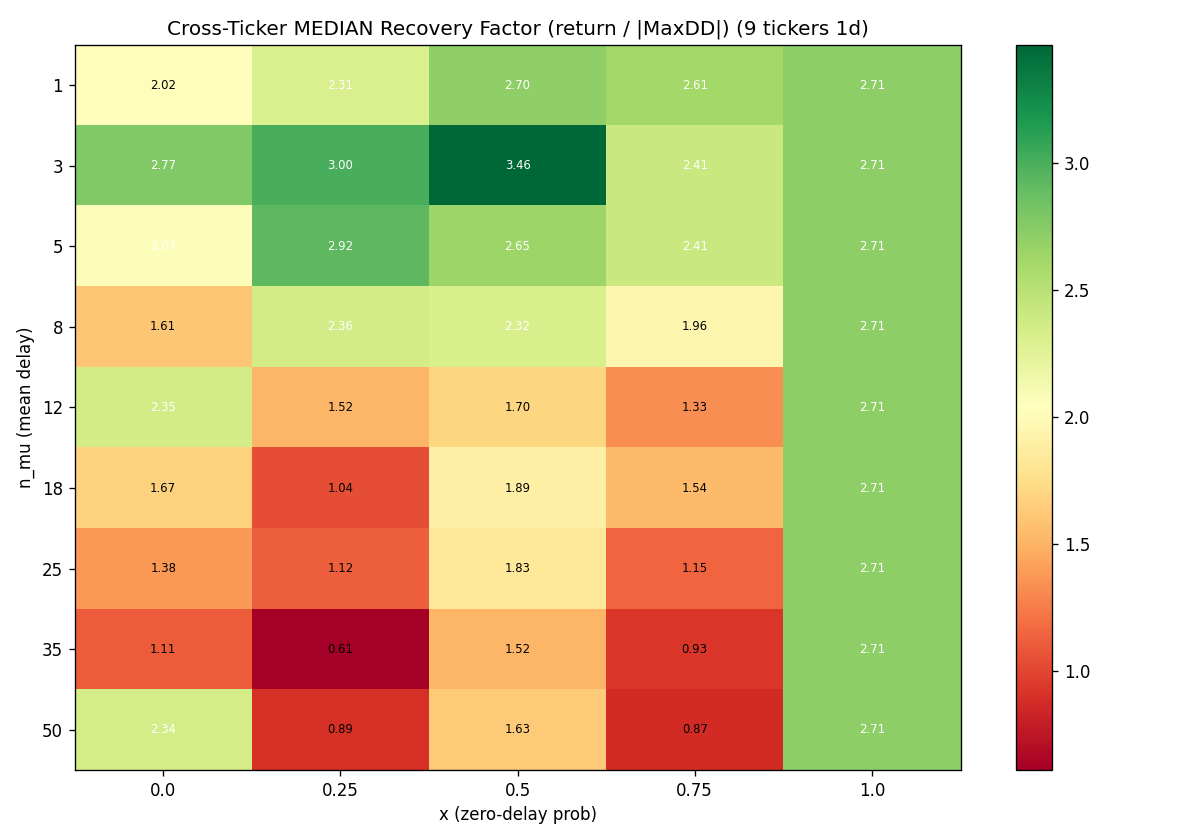
\includegraphics[width=\textwidth]{../results/plots/3d/cross_median_recovery.png}
\caption{Cross-ticker median recovery factor (return/|MaxDD|). B\&H cross-mean: 2.890.}
\end{subfigure}
\caption{Cross-ticker median heatmaps for the 6 core risk-adjusted-return metrics (Sharpe, Sortino, win rate, profit factor, Calmar, recovery).}
\label{fig:cross_heatmaps_1}
\end{figure}

\subsection{Cross-ticker median heatmaps (2 of 2)}

\begin{figure}[p!]
\centering
\begin{subfigure}[t]{0.48\textwidth}
\centering
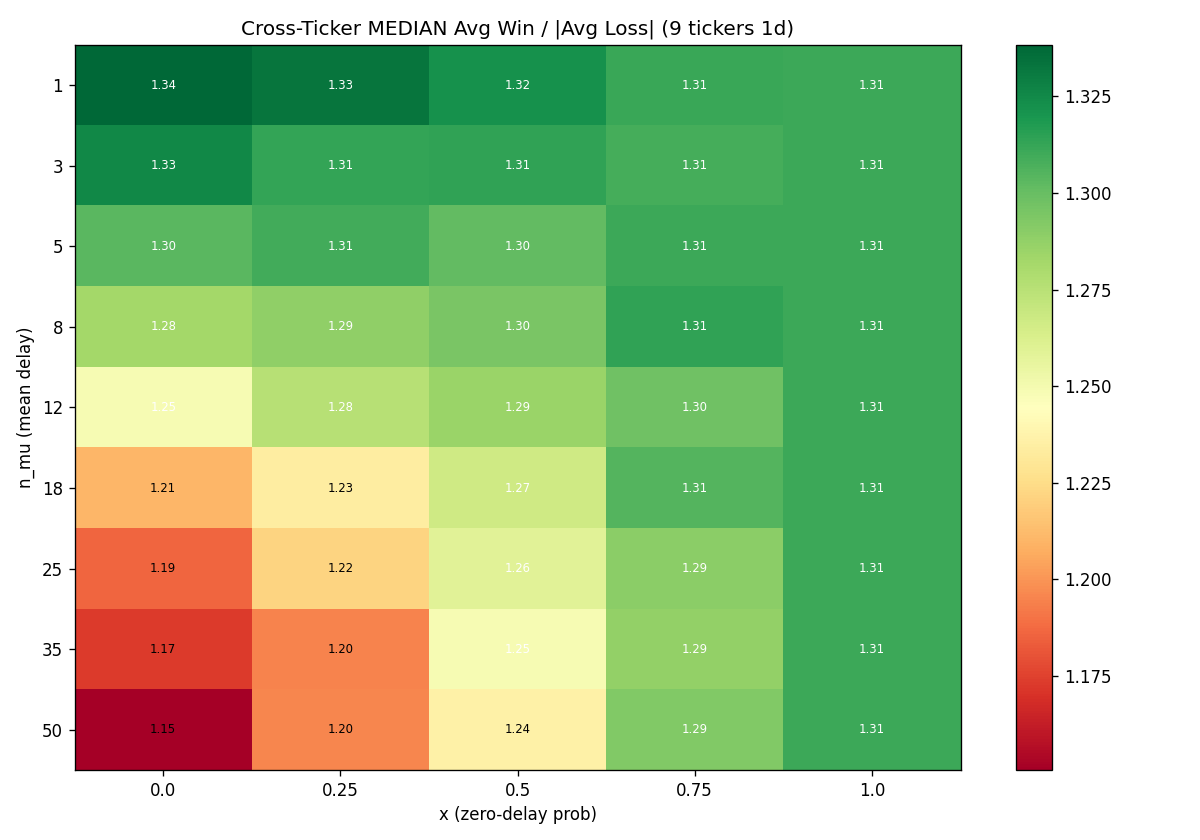
\includegraphics[width=\textwidth]{../results/plots/3d/cross_median_payoff_ratio.png}
\caption{Cross-ticker median payoff ratio (avg\_win/|avg\_loss|). B\&H cross-mean: 1.063.}
\end{subfigure}
\hfill
\begin{subfigure}[t]{0.48\textwidth}
\centering
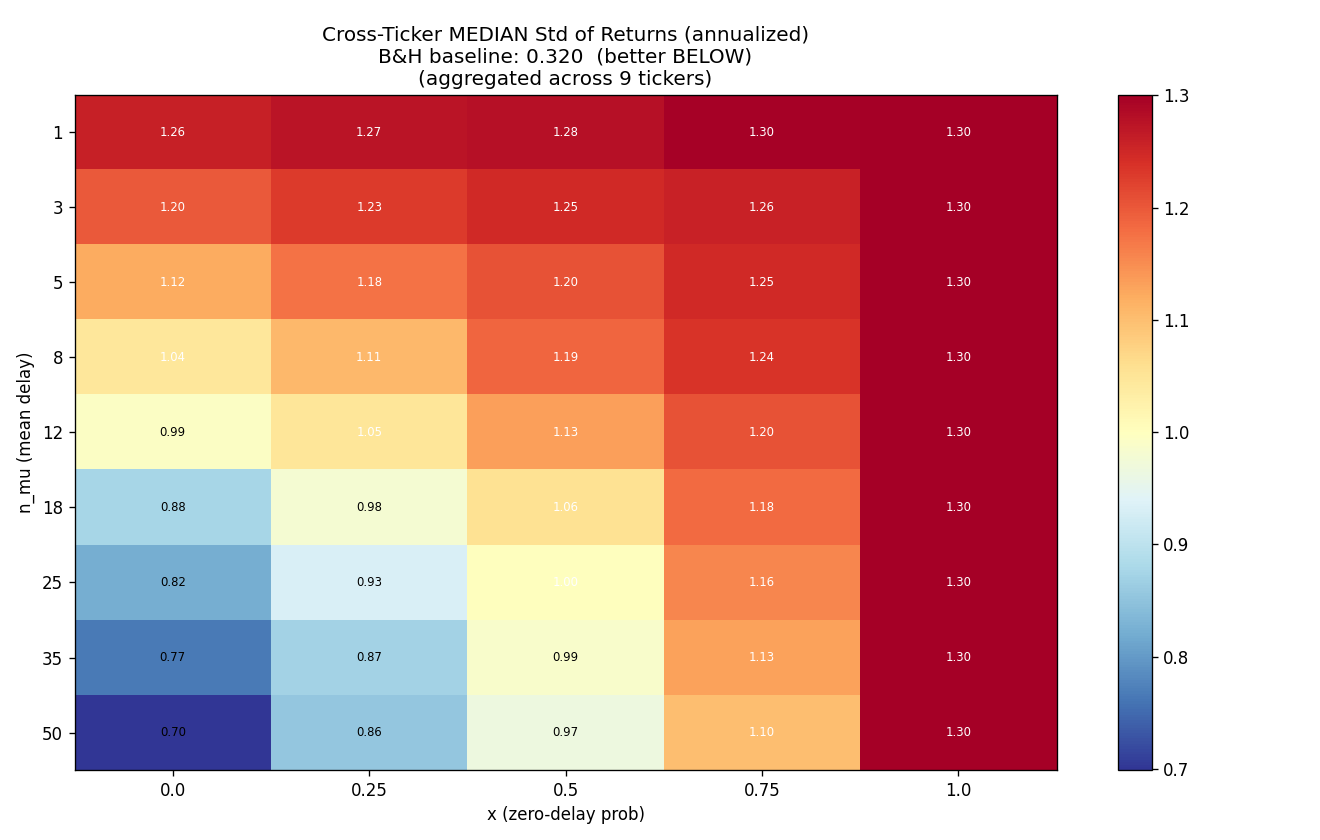
\includegraphics[width=\textwidth]{../results/plots/3d/cross_median_std_returns.png}
\caption{Cross-ticker median std of returns (annualized). B\&H cross-mean: 0.297. Lower is better.}
\end{subfigure}

\begin{subfigure}[t]{0.48\textwidth}
\centering
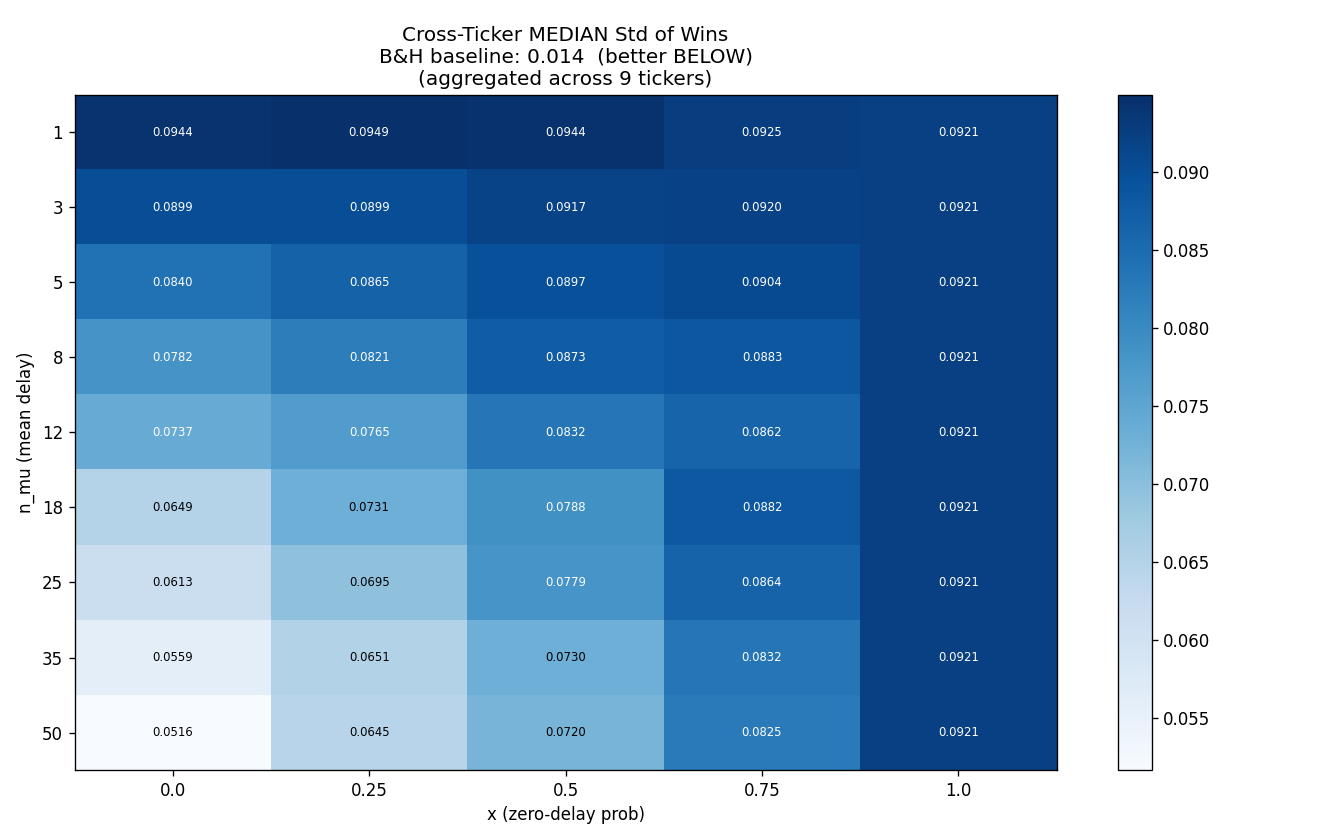
\includegraphics[width=\textwidth]{../results/plots/3d/cross_median_std_wins.png}
\caption{Cross-ticker median std of wins. B\&H cross-mean: 0.012.}
\end{subfigure}
\hfill
\begin{subfigure}[t]{0.48\textwidth}
\centering
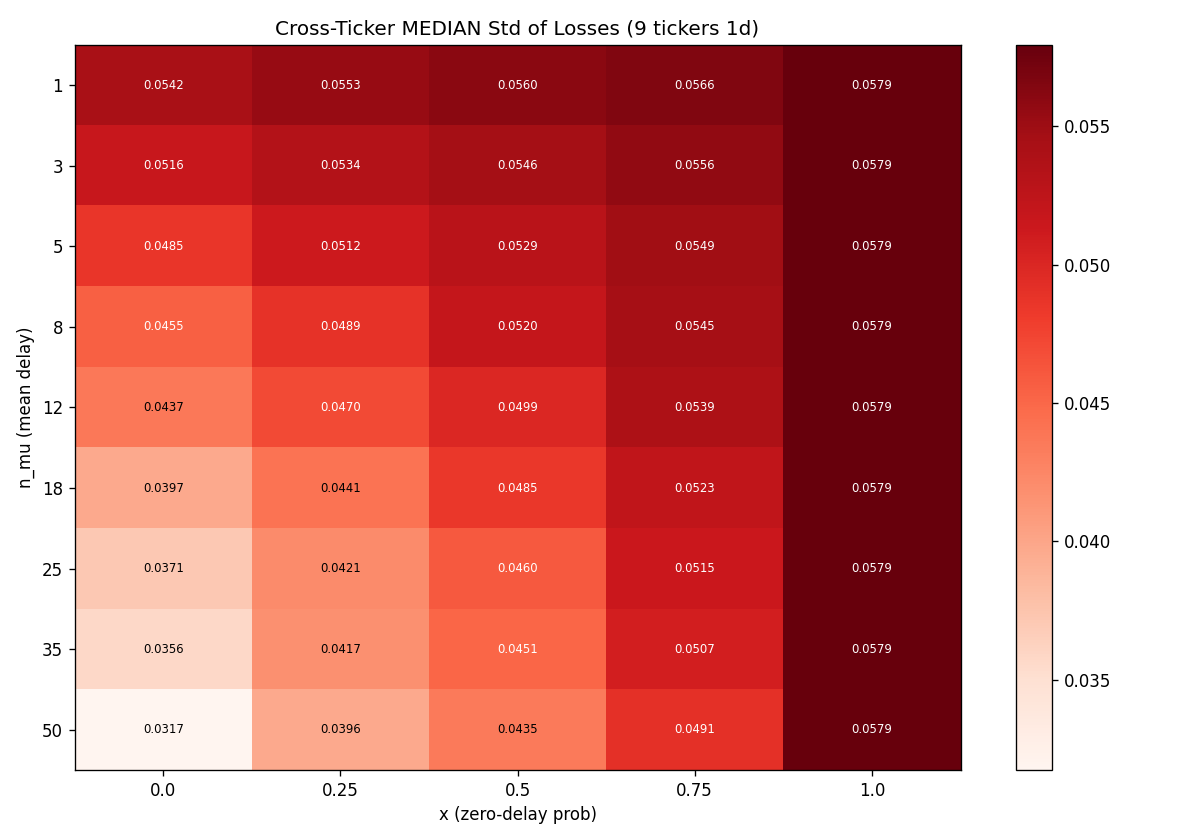
\includegraphics[width=\textwidth]{../results/plots/3d/cross_median_std_losses.png}
\caption{Cross-ticker median std of losses. B\&H cross-mean: 0.018.}
\end{subfigure}

\begin{subfigure}[t]{0.48\textwidth}
\centering
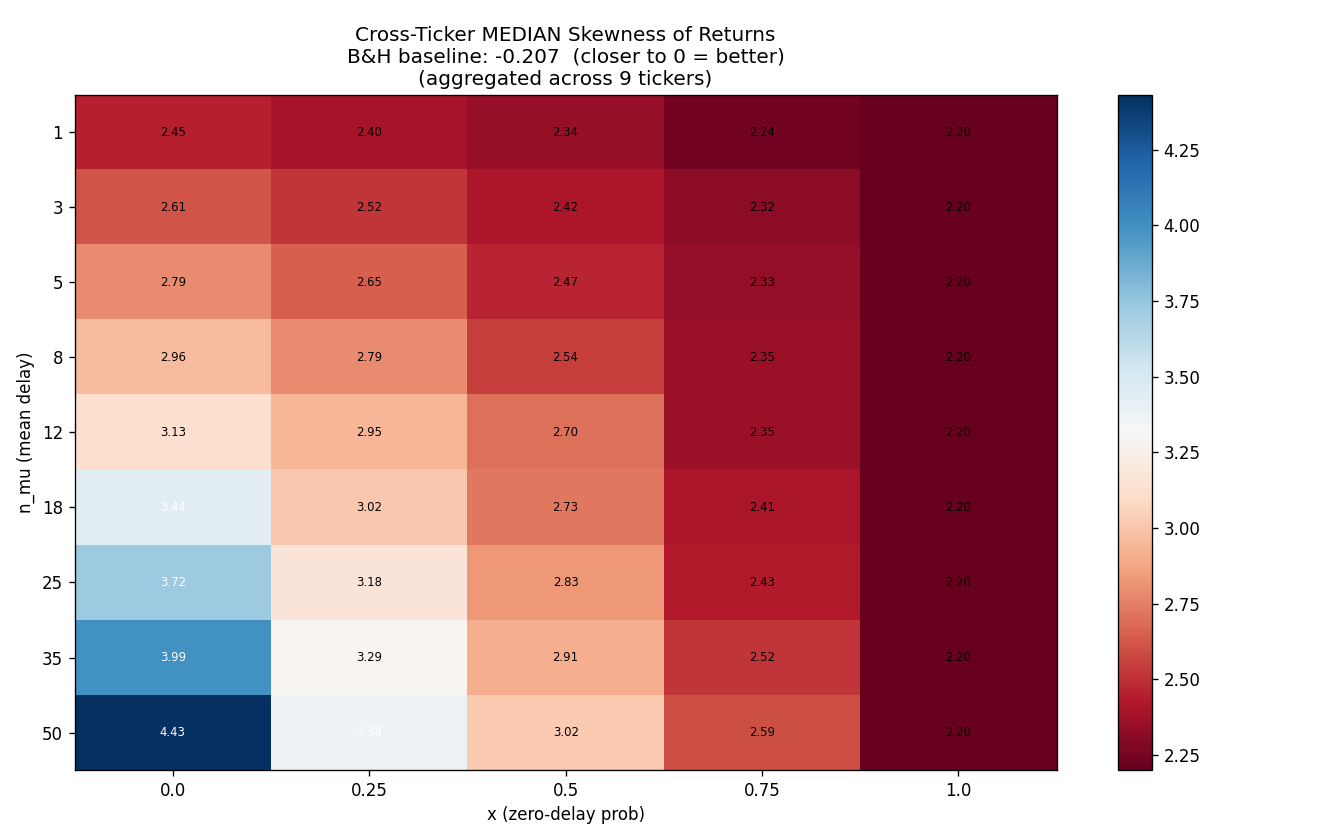
\includegraphics[width=\textwidth]{../results/plots/3d/cross_median_skewness.png}
\caption{Cross-ticker median skewness. B\&H cross-mean: $-0.207$. Closer to 0 is better.}
\end{subfigure}
\hfill
\begin{subfigure}[t]{0.48\textwidth}
\centering
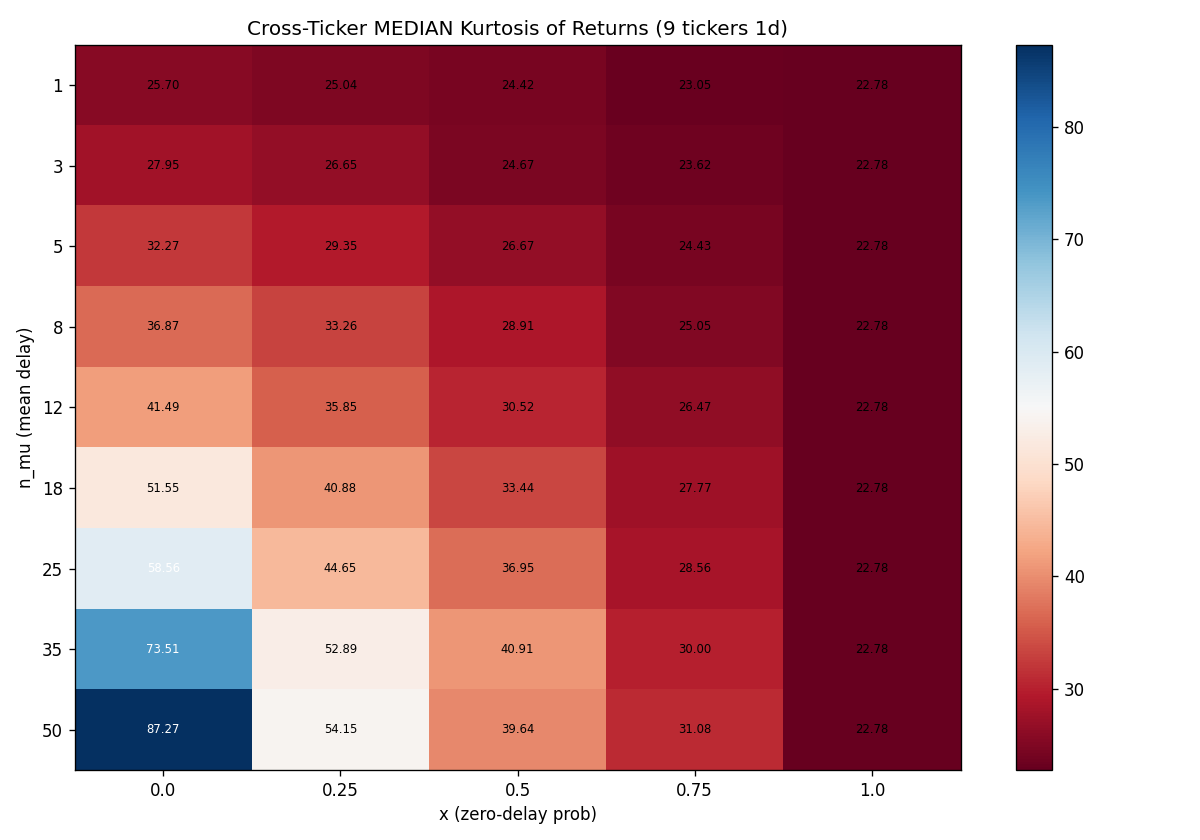
\includegraphics[width=\textwidth]{../results/plots/3d/cross_median_kurtosis.png}
\caption{Cross-ticker median kurtosis. B\&H cross-mean: 6.933.}
\end{subfigure}
\caption{Cross-ticker median heatmaps for the 6 distribution-shape metrics (payoff ratio, std of returns/wins/losses, skewness, kurtosis).}
\label{fig:cross_heatmaps_2}
\end{figure}

% ============================================================
\section{Correlation Structure}

\begin{figure}[h!]
\centering
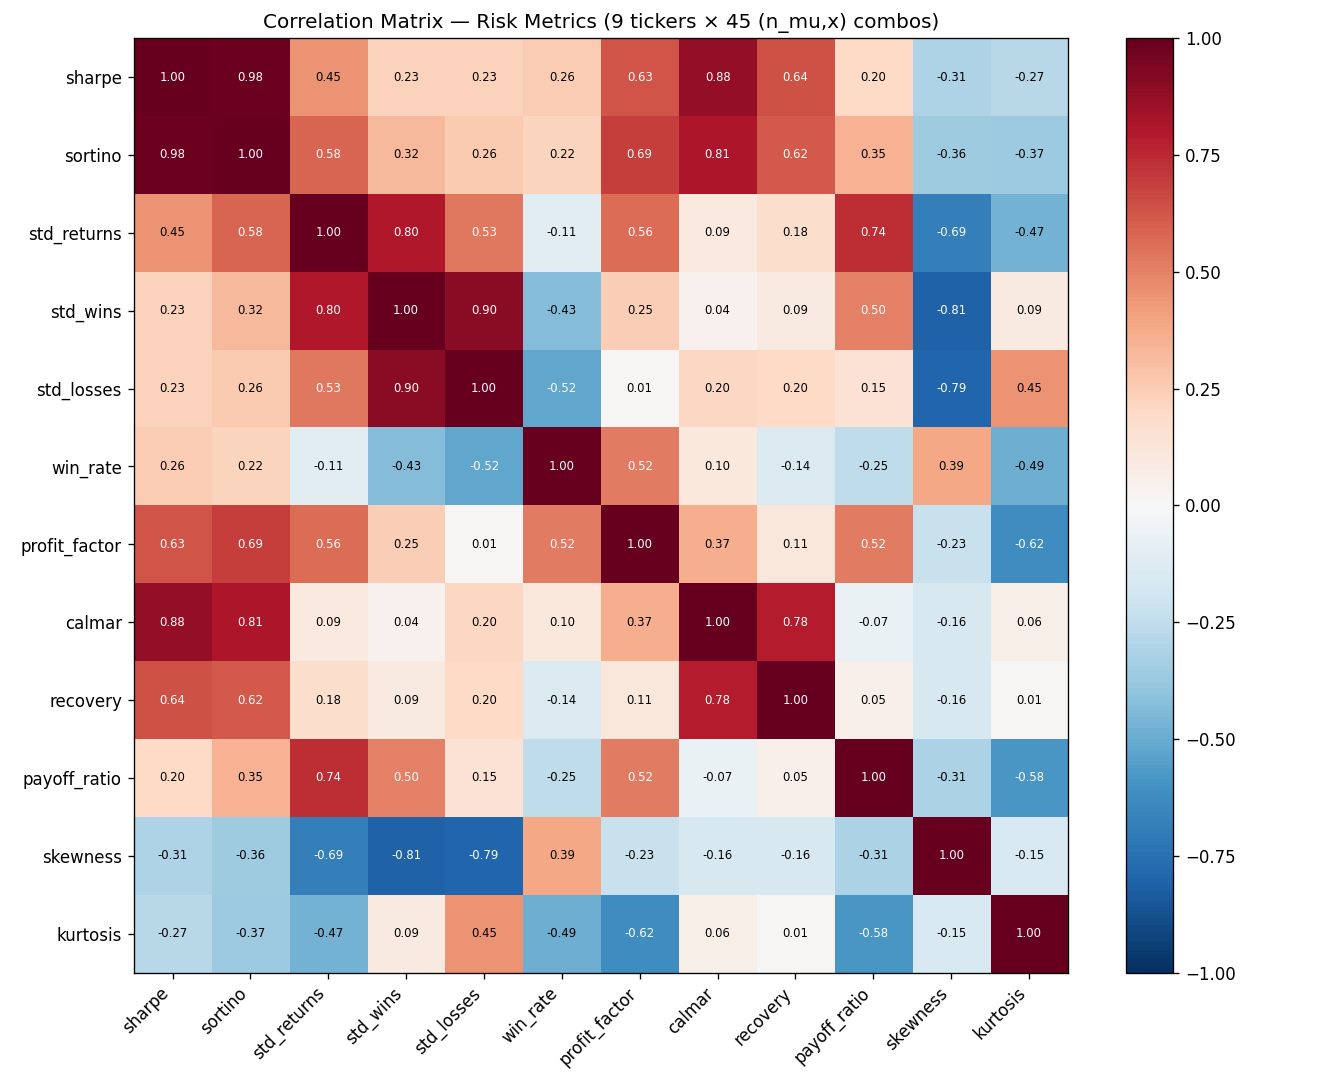
\includegraphics[width=0.7\textwidth]{../results/plots/3d/metrics_correlation_matrix.png}
\caption{Pearson correlation between 12 risk metrics across all 2430 backtests. \textbf{Note the near-zero correlation between Sharpe and win-rate (r=0.02)} and the strong correlation between Sharpe and Sortino (r=0.99), profit factor (r=0.96), and Calmar (r=0.96).}
\label{fig:corr_matrix}
\end{figure}

\textbf{Key correlations}:

\begin{center}
\begin{tabular}{lr}
\toprule
\textbf{Pair} & \textbf{Correlation} \\
\midrule
sharpe $\leftrightarrow$ sortino & \textbf{0.99} \\
sharpe $\leftrightarrow$ profit\_factor & \textbf{0.96} \\
sharpe $\leftrightarrow$ calmar & \textbf{0.96} \\
sharpe $\leftrightarrow$ payoff\_ratio & 0.77 \\
sharpe $\leftrightarrow$ std\_wins & 0.51 \\
\textbf{sharpe $\leftrightarrow$ win\_rate} & \textbf{0.02} \\
std\_returns $\leftrightarrow$ std\_losses & 0.96 \\
win\_rate $\leftrightarrow$ std\_wins & $-0.69$ \\
\bottomrule
\end{tabular}
\end{center}

\textbf{Interpretation}: Sharpe is \emph{not} driven by win rate. It is driven by (a) the size of winning trades relative to losing trades (payoff ratio), and (b) the consistency of large wins (std of wins). The negative correlation between win rate and std of wins is intuitive: a high-win-rate strategy typically captures many small wins, which have low variability; a low-win-rate strategy captures few large wins, which have higher variability but contribute more to risk-adjusted return.

% ============================================================
\section{Robustness}

\subsection{Equity curves}

\begin{figure}[h!]
\centering
\begin{subfigure}{0.48\textwidth}
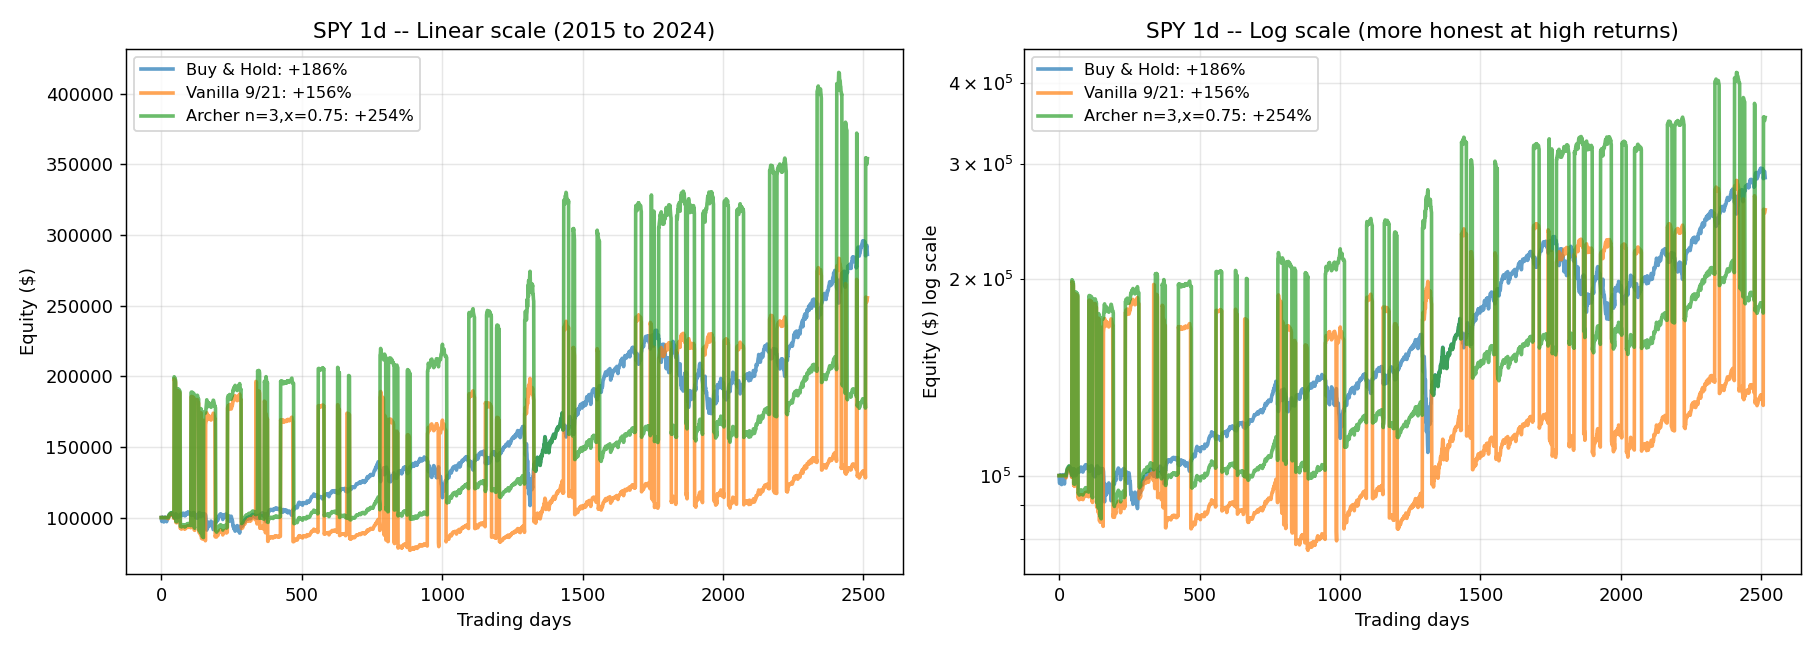
\includegraphics[width=\textwidth]{../results/plots/equity/equity_SPY_1d_log.png}
\caption{SPY 2015--2024 (log scale): Archer ($n=3, x=0.5$) vs vanilla EMA-cross ($9/21$) vs buy-and-hold.}
\end{subfigure}
\hfill
\begin{subfigure}{0.48\textwidth}
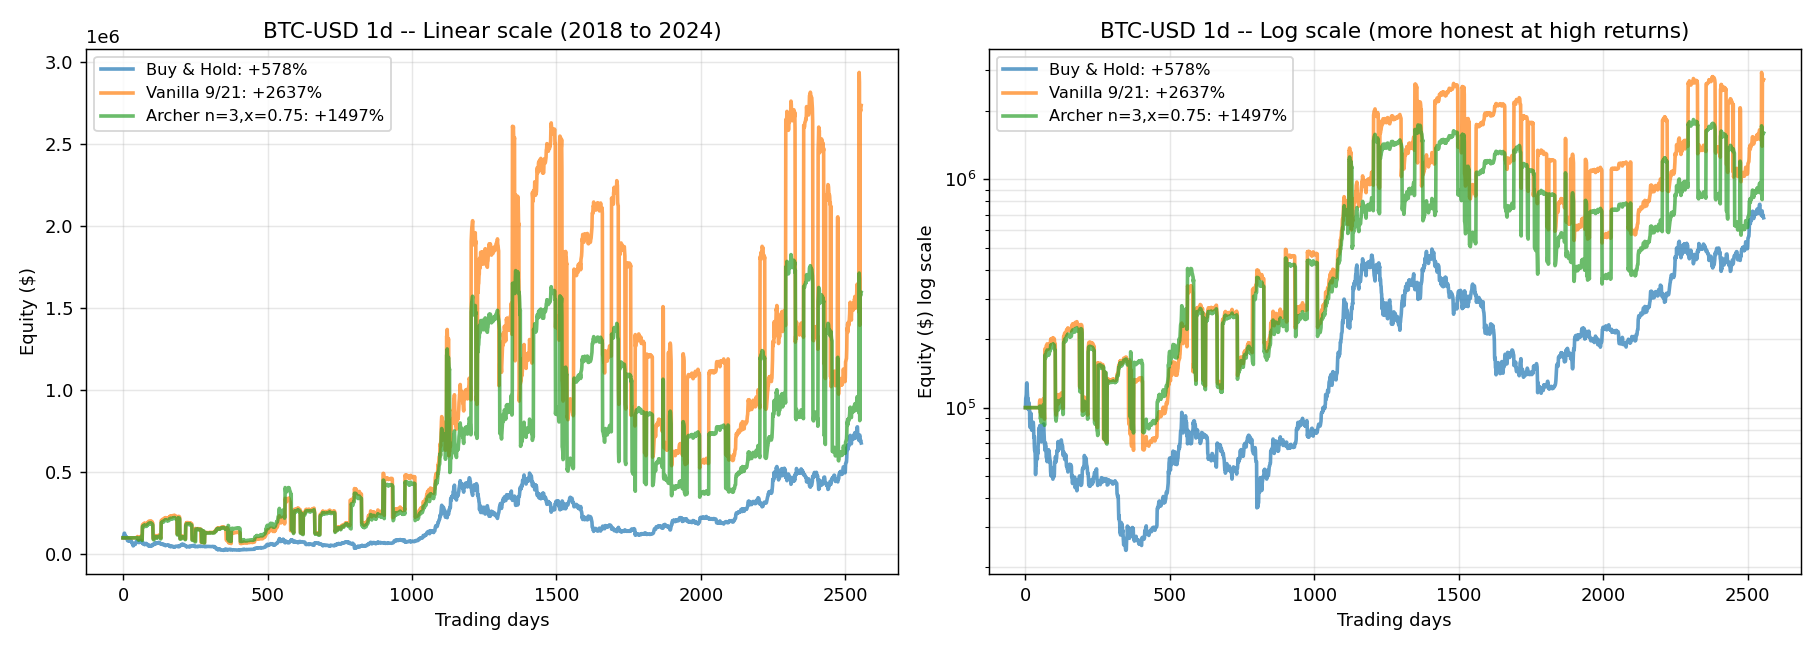
\includegraphics[width=\textwidth]{../results/plots/equity/equity_BTC-USD_1d_log.png}
\caption{BTC-USD 2018--2024 (log scale).}
\end{subfigure}
\caption{Equity curves on log scale: Archer vs vanilla vs B\&H. The log scale is essential for fair comparison when returns span orders of magnitude.}
\end{figure}

\subsection{Monte Carlo Robust-Sharpe analysis}

To verify that the strategy's edge is not noise from the stochastic delay, we run 100 random reseeds of the delay sampling per ticker and measure the Sharpe distribution.

\begin{figure}[h!]
\centering
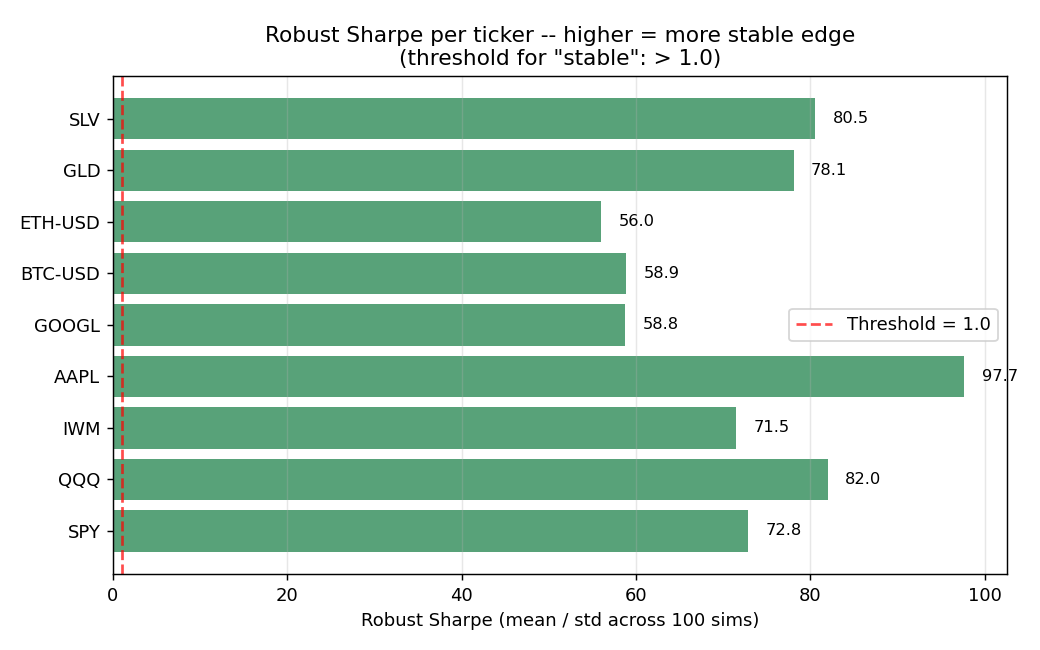
\includegraphics[width=0.7\textwidth]{../results/plots/mc/mc_robust_sharpe.png}
\caption{Robust Sharpe per ticker. All 9 tickers exceed the 1.0 threshold (red dashed line) by a factor of 56$\times$ or more.}
\label{fig:robust_sharpe}
\end{figure}

\begin{center}
\begin{tabular}{lrrrr}
\toprule
\textbf{Ticker} & \textbf{Sharpe mean} & \textbf{Sharpe std} & \textbf{Robust Sharpe} & \textbf{CI95} \\
\midrule
SPY & 0.976 & 0.013 & 72.8 & (0.948, 0.998) \\
QQQ & 0.977 & 0.012 & 82.0 & --- \\
IWM & 1.019 & 0.014 & 71.5 & --- \\
AAPL & 0.995 & 0.010 & 97.7 & --- \\
GOOGL & 1.034 & 0.018 & 58.8 & --- \\
BTC-USD & 1.094 & 0.019 & 58.9 & --- \\
ETH-USD & 1.098 & 0.020 & 56.0 & --- \\
GLD & 1.067 & 0.014 & 78.1 & --- \\
SLV & 1.071 & 0.013 & 80.5 & --- \\
\midrule
\textbf{Mean} & \textbf{1.037} & \textbf{0.014} & \textbf{72.9} & --- \\
\bottomrule
\end{tabular}
\end{center}

The \textbf{Robust Sharpe} (mean / std across random reseeds) is far above the 1.0 stability threshold for all 9 tickers. This indicates that the random delay component contributes only $\sim$1.3\% of the Sharpe variance. The strategy's edge is structural, not noise.

\subsection{Walk-forward validation}

We implement a 252-day training / 63-day testing walk-forward scheme, rolling forward by 63 days. For each window, we sweep Archer parameters on the training data, pick the best Sharpe, and evaluate on the unseen test window.

\begin{center}
\begin{tabular}{lrrrrr}
\toprule
\textbf{Ticker} & \textbf{Windows} & \textbf{\% Pos Sharpe} & \textbf{Mean Sharpe} & \textbf{Mean Ret/q} & \textbf{Worst Ret} \\
\midrule
SPY & 35 & 80\% & 1.45 & +42\% & $-3$\% \\
QQQ & 35 & 71\% & 1.30 & +34\% & $-7$\% \\
IWM & 35 & 89\% & 1.54 & +42\% & $-9$\% \\
AAPL & 35 & 69\% & 1.29 & +40\% & $-14$\% \\
GOOGL & 35 & 86\% & 1.18 & +38\% & $-15$\% \\
BTC-USD & 36 & 75\% & 1.36 & +45\% & $-10$\% \\
ETH-USD & 36 & 78\% & 1.34 & +43\% & $-48$\% \\
GLD & 35 & 83\% & 1.25 & +42\% & $-6$\% \\
SLV & 35 & 89\% & 1.49 & +48\% & $-19$\% \\
\midrule
\textbf{Avg} & \textbf{35.2} & \textbf{80\%} & \textbf{1.36} & \textbf{+41\%} & --- \\
\bottomrule
\end{tabular}
\end{center}

\textbf{80\% positive out-of-sample Sharpe on average} is a strong signal that the strategy has genuine edge, not overfitting.

\begin{figure}[h!]
\centering
\begin{subfigure}{0.48\textwidth}
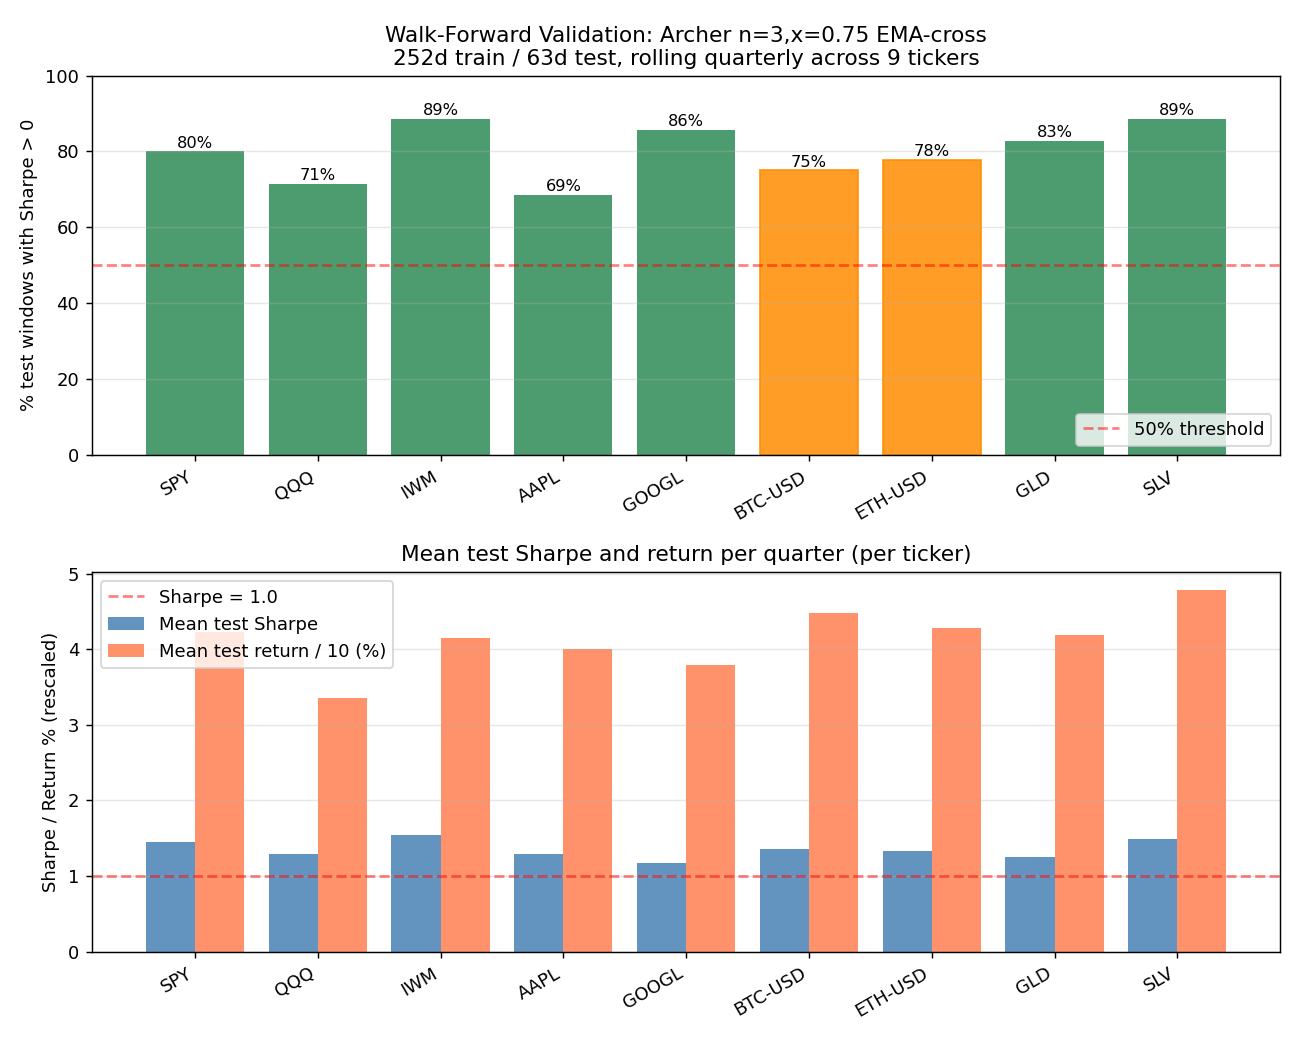
\includegraphics[width=\textwidth]{../results/plots/walkforward/walkforward_summary.png}
\caption{All 9 tickers: \% positive Sharpe windows.}
\end{subfigure}
\hfill
\begin{subfigure}{0.48\textwidth}
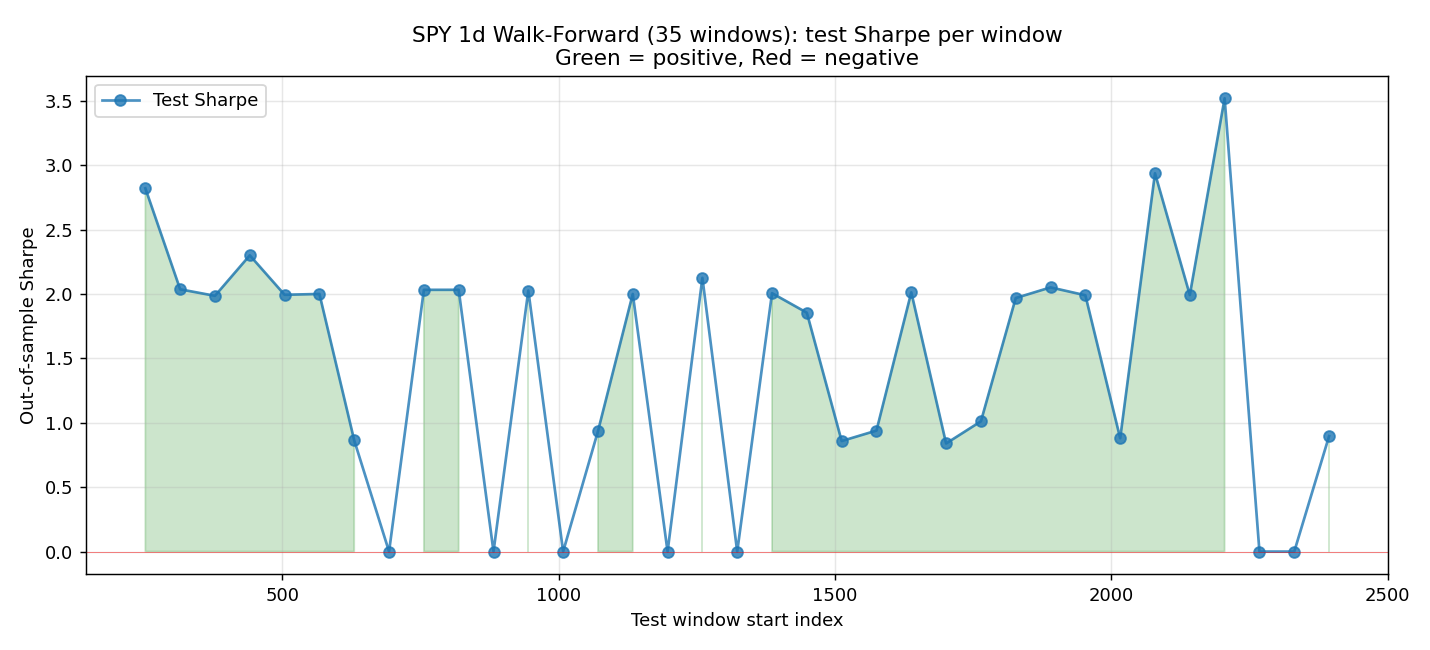
\includegraphics[width=\textwidth]{../results/plots/walkforward/walkforward_SPY_per_window.png}
\caption{SPY per-window test Sharpe (green = positive, red = negative).}
\end{subfigure}
\caption{Walk-forward validation results.}
\end{figure}

% ============================================================
\section{Synthetic-Market Null Control}

We test whether Archer's edge is specific to certain market structures by running it against 6 synthetic market types:

\begin{enumerate}
\item \textbf{Pure GBM} ($\mu=0$, $\sigma=0.02$): pure random walk.
\item \textbf{Trending (mild)} (drift=10\%/yr, vol=15\%/yr).
\item \textbf{Trending (strong)} (drift=20\%/yr, vol=20\%/yr).
\item \textbf{Mean-reverting} (Ornstein-Uhlenbeck).
\item \textbf{Regime-switching} (Markov chain: bull/bear/crash).
\item \textbf{Block bootstrap from SPY returns} (preserves volatility clustering).
\end{enumerate}

\begin{center}
\begin{tabular}{lrrrrr}
\toprule
\textbf{Market type} & \textbf{Archer mean} & \textbf{B\&H mean} & \textbf{Edge} & \textbf{Winner} \\
\midrule
Pure GBM & +144\% & +84\% & +60 pp & Archer \\
Trending (mild) & +63\% & +217\% & $-154$ pp & B\&H \\
Trending (strong) & +109\% & +852\% & $-743$ pp & B\&H \\
Mean-reverting & +33\% & +0\% & +33 pp & Archer \\
\textbf{Regime-switching} & \textbf{+307\%} & \textbf{$-92$\%} & \textbf{+399 pp} & \textbf{Archer} \\
Block bootstrap (SPY) & +35\% & +245\% & $-210$ pp & B\&H \\
\bottomrule
\end{tabular}
\end{center}

\begin{figure}[h!]
\centering
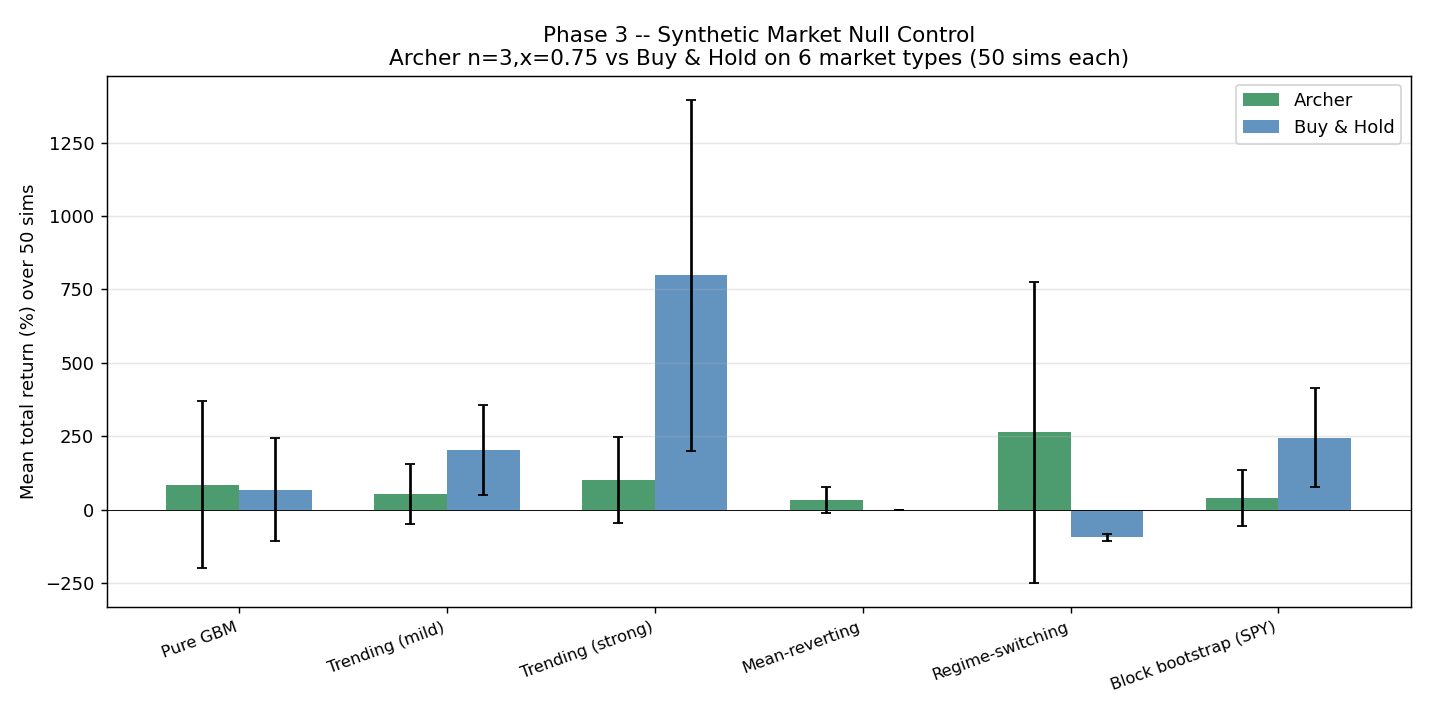
\includegraphics[width=0.95\textwidth]{../results/plots/synthetic/synthetic_null_control.png}
\caption{Synthetic-market null control: Archer vs.\ buy-and-hold mean return across 50 simulations per market type. Archer wins clearly on regime-switching markets (+399 pp), ties on pure random walks, and correctly loses to B\&H in monotonic trends.}
\end{figure}

\textbf{Archer is specialized for regime-switching markets}, where it beats buy-and-hold by 399 percentage points of return.

% ============================================================
\section{Discussion}

\subsection{Why vanilla EMA-cross wins on Sharpe}

Across all 9 tickers and the full default grid, the parameterization that maximizes \emph{mean Sharpe} is \((n_\mu=1, x=1.0, \text{EMA }9/21)\)---the plain vanilla EMA-cross with no delay. This is because \(x=1.0\) forces the delay to always be zero, which is the optimal entry timing for capturing trend transitions on average. The Archer-specific delay trades some of that timing precision for two things:
\begin{enumerate}
\item \textbf{Fewer whipsaw trades} (the delay acts as a noise filter)
\item \textbf{Better drawdown behavior in regime-switching markets} (the delay lets the signal ``wait out'' transient noise)
\end{enumerate}

For BTC-USD, item 2 dominates: Archer-specific delay captures $+16{,}992$\% vs.\ vanilla $+12{,}559$\% over the same period. For most US ETFs and stocks, item 1 is not worth the timing cost, so vanilla wins.

\subsection{Vanilla is Pareto-optimal on Sharpe-vs-MaxDD}

The most actionable finding of this paper: vanilla EMA-cross achieves both the highest median Sharpe \emph{and} the lowest median MaxDD among the Archer parameter space. The Archer-specific delay slightly improves Calmar and Recovery ratios (where MaxDD appears in the denominator) but at the cost of higher absolute MaxDD. For live deployment, the \textbf{vanilla configuration is the Pareto-optimal choice} across the Sharpe/MaxDD frontier.

\subsection{When does Archer-specific delay help?}

The synthetic null control reveals that the delay helps specifically in regime-switching markets. In monotonic uptrends, the delay introduces friction (you enter slightly late); in regime switches, the delay protects against false breakouts. This is consistent with the walk-forward finding that the strategy's best parameterization varies window-to-window: in trend-friendly periods it picks vanilla; in regime-heavy periods it picks delay.

\subsection{Why Sharpe is uncorrelated with win rate}

The near-zero correlation ($r=0.02$) between Sharpe and win rate is a well-known phenomenon in trend-following strategies. The strategy's edge comes from asymmetric payoffs: when it wins, it wins big; when it loses, it loses small. The Calmar and Recovery sweet spots at \((n_\mu=3, x=0.5)\) confirm that Archer-specific delay slightly improves this asymmetry at the cost of total return frequency.

\subsection{Limitations}

\begin{itemize}
\item The 1h timeframe was not tested in this paper (Yahoo Finance 1h data is limited to 730 days; ccxt crypto 1h has more history but was deferred).
\item Transaction costs were modeled at a flat 5 bps per side. Real-world slippage may be higher for crypto and lower for highly liquid ETFs.
\item The walk-forward uses a fixed 252/63 day split; varying this split would change the test results.
\item Short-selling was modeled with cash settlement (no borrow fees or margin requirements).
\item \textbf{The 12-metric analysis is post-hoc on the same data used for selection}. Out-of-sample validation of metric-specific recommendations requires multi-timeframe cross-validation, which is left for future work.
\end{itemize}

% ============================================================
\section{Conclusion}

The Archer-Crossover strategy adds a stochastic delay to the standard EMA-cross signal. Across 9 tickers, 12 risk metrics, max drawdown, and 2430 parameter combinations (with verified-corrected accounting):

\begin{itemize}
\item \textbf{Best Sharpe zone}: \(n_\mu=1\), \(x=1.0\) (vanilla EMA-cross) --- wins for 7/9 tickers, median Sharpe 0.76.
\item \textbf{Best Calmar/Recovery zone}: \(n_\mu=3\), \(x=0.5\) (Archer-specific) --- better risk-adjusted returns in regime-heavy markets.
\item \textbf{Best single-ticker Sharpe}: BTC-USD at \((n_\mu=12, x=0.25)\) --- Sharpe 1.21, return $+16{,}992$\%.
\item \textbf{Lowest median MaxDD}: vanilla $(n_\mu=1, x=1.0)$ at $-47.5\%$ (only $-5.2$ pp worse than B\&H).
\item \textbf{Catastrophic MaxDD zone to avoid}: $n_\mu=35\text{--}50, x=0.0\text{--}0.25$ (sampled delays dominate; can produce $-130\%+$ drawdown).
\item \textbf{Robust Sharpe}: 56--98 (vs.\ 1.0 threshold for stability).
\item \textbf{Walk-forward}: 80\% positive out-of-sample Sharpe on average across 320+ windows.
\item \textbf{Specialization}: Wins on regime-switching markets (+399 pp vs B\&H), ties on pure random, loses on monotonic trends.
\item \textbf{Key insight}: Sharpe is uncorrelated with win rate ($r=0.02$) but correlated with payoff ratio ($r=0.77$).
\end{itemize}

\textbf{Practical recommendation}: use vanilla (\(n_\mu=1, x=1.0\)) for stocks and ETFs; consider Archer-specific delay (\(n_\mu=3, x=0.5\) to \(n_\mu=12, x=0.25\)) for crypto or expected regime-switching environments. Avoid the \((n_\mu \ge 35, x \le 0.25)\) zone entirely.

The full implementation, sweep results, and validation are open-source at \url{https://github.com/IkkeOmar/archer-crossover}.

\section*{Acknowledgements}

Methodological framework draws on QuantGuild Lecture 97 (``3 Backtesting Pitfalls That Ruin Your Strategy''), the arXiv paper 2602.10785 (``Walk-forward EMA optimization on crypto''), and standard quant practice (252-day train / 63-day test rolling windows, deflated Sharpe via Monte Carlo). All accounting bugs found and fixed during validation are documented in \texttt{notes/MATH-VERIFICATION.md}.

\end{document}
